\documentclass[runningheads]{llncs}

\usepackage{amssymb}
\usepackage{amsmath}
\usepackage{float}
\usepackage{fancyvrb}
%% The amsthm package provides extended theorem environments

% \usepackage{amsthm}
% AM commented out because it clashes with proof, etc

%% The lineno packages adds line numbers. Start line numbering with
%% \begin{linenumbers}, end it with \end{linenumbers}. Or switch it on
%% for the whole article with \linenumbers.
\usepackage{lineno}

%% Use package enumitem to align enumeration and itemization
\usepackage{enumitem}
\usepackage{listings}
%\usepackage{courier}           % for the courier font (optional)
\usepackage{multicol}          % for two equations side by side
\usepackage[justification=centering]{caption}
\usepackage[dvipsnames]{xcolor}
\usepackage{stmaryrd}
\usepackage{hyperref}
%\usepackage{cleveref}
\usepackage{hieroglf}
\usepackage{scalerel}
\usepackage{tikz}
\usepackage{pgfplots}
\usepackage[export]{adjustbox} % for subfigures
\usepackage{semantic}          % for mathlig


\hypersetup{ % play with these to change the look of hyperlinks
	colorlinks=true,
	linkcolor=black,
	filecolor=magenta,
	urlcolor=blue,
	citecolor=black
}

\newcommand{\coq}{\scalebox{.6}{\textpmhg{\Ha}}}
\newcommand{\p}[1]{\ensuremath{\mathsf{#1}}} % predicate font
\newcommand{\m}[1]{\ensuremath{\mathit{#1}}} % math font
\newcommand{\braces}[1]{\left\{\begin{array}{l@{}} #1 \end{array}\right\}}
\let\ramify\lightning
\newcommand{\sz}{\texttt{SIZE}}
\newcommand{\ifty}{\texttt{INF}}
\newcommand{\defeq}{\mathbin{\stackrel{\Delta}{=}}}
\newcommand{\bigO}{\text{O}}
\usetikzlibrary{shadows}
\usetikzlibrary{arrows.meta, positioning, decorations.pathmorphing, fit, matrix}
\mathlig{/|}{\mathbin{\wedge}} % additive conjunction


% required by LNCS
\renewcommand\UrlFont{\color{blue}\rmfamily}

\colorlet{red}{red!80!black}
\colorlet{green}{green!50!black}

%% NEW COMMANDS =============================================

\lstdefinestyle{myStyle}{
	%	language=Coq,
	keywords={Inductive,Require,Import,Definition,Fixpoint,match,with,end,let,in,fix},
	basicstyle=\normalfont\footnotesize\tt,
	keywordstyle=\color{green}, % Blue clashes with the cyan links. Change if you want.
	stepnumber=1,
	tabsize=2,
	numbers=none,
	numberstyle=\tiny,
	numbersep=5pt,
	showspaces=false,
	escapechar=`,
	showstringspaces=false
}
%basicstyle=\fontsize{10}{11}\selectfont\ttfamily,

\lstdefinestyle{myTinyStyle}{
	%   language=Coq,
	basicstyle=\normalfont\fontsize{7.0}{7.3}\tt,
	stepnumber=1,
	tabsize=2,
	numbers=none,
	numberstyle=\tiny,
	numbersep=5pt,
	showspaces=false,
	showstringspaces=false,
	language=C,
	morecomment=[l][{\color{OliveGreen}}]{//},
	sensitive=true,
	mathescape=true,
	showlines=true,
	escapechar=`,
	basicstyle=\footnotesize\ttfamily,
	keywordstyle=\color{blue}, numbers=left,
	numberstyle=\tiny, numbersep=5pt, boxpos=t
}

\lstdefinestyle{CoqStyle}{
%	language=Coq,
    keywords={forall,Prop,Type,Inductive,Require,Import,Definition,Fixpoint,match,with,end,let,in,fix,if,then,else},
	basicstyle=\footnotesize\ttfamily,
    keywordstyle=\color{blue},
	stepnumber=1,
	tabsize=2,
    numbers=none,
    numberstyle=\tiny,
    numbersep=5pt,
	showspaces=false,
    escapechar=`,
	showstringspaces=false
}

\lstset{style=myTinyStyle}
\makeatletter
\newlength{\@mli}
\newcommand{\mli}[1]{%
	\settowidth{\@mli}{\lstinline/#1/}
	\hspace{-.5ex}\begin{minipage}[t]{\@mli}\lstinline/#1/\end{minipage}}
\makeatother
\newcommand{\li}[1]{\ifmmode\mbox{\mli{#1}}\else\mbox{\lstinline/#1/}\fi}

\newcommand\hide[1]{}

\newenvironment{centermath}
{\begin{center}$\displaystyle}
	{$\end{center}}

\renewcommand{\note}[2][polish]{{\color{red} #2}{\marginpar{\tiny \color{blue} #1}}}
\renewcommand{\implies}{\Rightarrow}
\renewcommand{\iff}{\Leftrightarrow}

\title{Functional Correctness of C implementations \\
of Dijkstra's, Kruskal's, and Prim's Algorithms}
\titlerunning{Functional Correctness of Dijkstra's, Kruskal's, and Prim's Algorithms}
%optional, please use if title is longer than one line

\begin{document}

\hide{
	\author{Anshuman Mohan \and
	Wei Xiang Leow \and
%	Shengyi Wang\inst{2} \and
	Aquinas Hobor} %\inst{1,2}}

	%\authorrunning{A. Mohan et al.}
% First names are abbreviated in the running head.
% If there are more than two authors, 'et al.' is used.
	
	\institute{National University of Singapore}% \and
%	Princeton University, USA \and
%	Yale-NUS College, National University of Singapore}	
}
\author{ } \institute{ }
	\maketitle
	%\begin{frontmatter}
	
	%% Title, authors and addresses
	
	%% use the tnoteref command within \title for footnotes;
	%% use the tnotetext command for theassociated footnote;
	%% use the fnref command within \author or \address for footnotes;
	%% use the fntext command for theassociated footnote;
	%% use the corref command within \author for corresponding author footnotes;
	%% use the cortext command for theassociated footnote;
	%% use the ead command for the email address,
	%% and the form \ead[url] for the home page:
	
	%% \tnotetext[label1]{}
	%% \author{Name\corref{cor1}\fnref{label2}}
	%% \ead{email address}
	%% \ead[url]{home page}
	%% \fntext[label2]{}
	%% \cortext[cor1]{}
	%% \address{Address\fnref{label3}}
	%% \fntext[label3]{}
	
	%% use optional labels to link authors explicitly to addresses:
	%% \author[label1,label2]{}
	%% \address[label1]{}
	%% \address[label2]{}
	
	%\author{}
	
	%\address{}
	\vspace{-2em}
	
	\begin{abstract}
		\vspace{-1.2em}
        We develop machine-checked verifications of the full functional correctness of C implementations of the eponymous graph algorithms of Dijkstra, Kruskal, and Prim.  We extend Wang et al's CertiGraph platform \cite{DBLP:journals/pacmpl/WangCMH19} to reason about labels on edges, undirected graphs, and common spatial representations of edge-labeled graphs such as adjacency matrices and edge lists.  We certify binary heaps, including Floyd's bottom-up heap construction, heapsort, and increase/decrease priority.
        Our verifications uncover subtle overflows implicit in standard textbook code, including a nontrivial bound on edge weights necessary to execute Dijkstra's algorithm: in fact, we show that the intuitive guess fails and provide a workable refinement.  We observe that the common notion that Prim's algorithm requires a connected graph is wrong: we verify that a standard textbook implementation of Prim's algorithm can compute minimum spanning forests without finding components first.  Our verification of Kruskal's algorithm is notable because it requires reasoning about two graphs simultaneously: the undirected graph undergoing MST construction, and the directed graph representing the forest inside union-find.  Our binary heap verification exposes precise bounds for the heap to operate correctly, avoids a subtle overflow error, and includes a method of recycling keys to avoid overflow. %heap requires 0u, etc.?
		\keywords{separation logic \and graph algorithms \and Coq \and VST}
%Dijkstra's shortest-path \and Prim's algorithm \and Kruskal's algorithm \and minimum spanning trees \and verification \and CompCert \and VST}
	\end{abstract} %\and Coq
	
	%\end{frontmatter}
	
	%% \linenumbers
	
	%% main text
%\hide{	
	\section{Introduction}
	\label{sec:intro}
	Dijkstra's eponymous shortest-path algorithm~\cite{Dijk} finds
the cost-minimal paths from a distinguished \emph{source} vertex
source to all reachable vertices in a finite directed graph.

The algorithm is classic and ubiquitous, appearing widely in textbooks
and in real routing protocols. Further, the algorithm has been in
use for over $60$ years, suggesting, for all practical purposes,
that its safety and correctness have been verified by decades of application.

Recent efforts [cite Mizar, cite ACL2, cite Coq] have implemented the algorithm
in proof assistants and formally proved claims about its behavior.
However, because they operate entirely within idealized formal checkers,
these works inadvertently gloss over certain classes of issues
that routinely crop up in real-world settings.

In this paper we verify a~C~implementation of Dijkstra's
one-to-all shortest path algorithm. We implement
textbook~C~code [cite CLRS], import it into Coq [cite VST],
and state and prove a correctness claim in Coq [cite VST, cite RamifyCoq].
We expose a subtle overflow issue in the code, and address the issue
via a nontrivial refinement in the precondition of the algorithm.

The paper is organized as follows:
\vspace{-1em}
\begin{itemize}
    \item[\S\ref{sec:overview}] We briefly present and explain
    our~C~implementation of Dijkstra's algorithm.
    \item[\S\ref{sec:verification}] We present our specification
    and our most important loop invariant.
    \item[\S\ref{sec:overflow}] We explain the critical overflow issue
    in the code, and propose a fix by refinining the specification.
\end{itemize} 
	
	\subsection{I'm sorry Dave, I'm afraid I can't do that: Overflow}
	\label{sec:overflow}
	Dijkstra's algorithm clearly cannot work when a path
cost is greater than \texttt{INT\_MAX}.  A reasonable-looking restriction 
is to bound edge costs by 
$\left\lfloor\frac{\texttt{INT\_MAX}}{\texttt{size}-1}\right\rfloor$, since 
the longest optimal path has $\texttt{size}-1$ links and so the 
most expensive possible path costs no more than \texttt{INT\_MAX}.  
However, this has two flaws.  First, since we are writing real code in~C, 
rather than pseudocode in an idealized setting, we must reserve some 
concrete \texttt{int} value \texttt{inf} for ``infinity'', which has 
the special semantics that, if the best-known distance to a vertex~\m{x}
is \texttt{inf}, then~\m{x} is as-yet unreachable. 
A consequence of this is that reachable destination vertices cannot have a 
path cost of \texttt{inf}: if they did, this would be logged in the 
\m{dist} array and create an unpleasant ambiguity. 
Second, even though the best-known distances start at \texttt{inf} 
(see line~\ref{code:assigninf}) and only ever decrease from there, the code can 
overflow on lines~\ref{code:overflow}~and~\ref{code:update1}.

\begin{figure}[t]
\centering
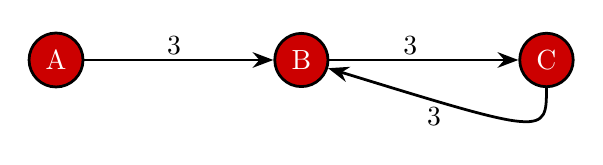
\begin{tikzpicture}[x=0.3cm, y=0.3cm,
  vert/.style={circle, line width=1pt, draw, fill=red}]
  \node[vert] (A) at (0,0) {\color{white}A};
  \node[vert] (B) [right = 8 of A] {\color{white}B};
  \node[vert] (C) [right = 8 of B] {\color{white}C};
  \draw [->,line width=1pt,arrows={-Stealth}] (A) -- (B);
  \draw [->,line width=1pt,arrows={-Stealth}] (B) -- (C);
  \draw [->,line width=1pt,arrows={-Stealth}] (C.south) .. controls ++(0, -2) .. (B);
  \node at (5,0.6) {3};
  \node at (15,0.6) {3};
  \node at (16,-2.4) {3};
\end{tikzpicture}
\caption{A graph that will result in overflow on a 3-bit machine.}
\label{fig:overflow}
\end{figure}

Consider applying Dijkstra's algorithm on a hypothetical 3-bit unsigned machine to 
the graph in figure~\ref{fig:overflow}.  The \texttt{size} of the graph is 3 nodes, and so the na\"ive edge-weight upper bound is $\left\lfloor\frac{\texttt{INT\_MAX}}{\texttt{size}-1}\right\rfloor = \left\lfloor\frac{7}{3-1}\right\rfloor = 3$, exactly as pictured in figure~\ref{fig:overflow}.  Indeed, a glance at the diagram is enough to tell that the true distance from the source~A~to vertices~B~and~C~are~3~and~6 respectively---both of which are representable with 3 bits, and so na\"ively all seems well.  %Unfortunately, Dijkstra's algorithm does not exactly work like that.  
Indeed, after processing vertices~A~and~B, 3~and~6~\emph{are} the costs reflected in the \m{dist} array for~B~and~C respectively---\emph{but unfortunately vertex~C~is still in the priority queue}.  After vertex~C~is popped on line~\ref{code:pop}, we fetch its neighbors in the \texttt{for} loop; vertex~B's cost of~3~is fetched on line~\ref{code:cost}.  On line~\ref{code:overflow} the currently optimal cost of~B~(3) is compared against the sum of the optimal cost of~C~(6) plus the just-retrieved cost of the edge from~C~to~B~(3).  Since $6+3$ overflows in 3-bit arithmetic, the comparison is not between~3~and~9 but in fact between~3~and~1!  Thus the code decides that a new cheaper path from~A~to~B~exists (in particular, A$\leadsto$B$\leadsto$C$\leadsto$B) and then trashes the \texttt{dist} and \texttt{prev} arrays on line~\ref{code:update1}.  %

Our code uses signed \texttt{int} rather than \texttt{unsigned int} so we have undefined behavior rather than defined-but-wrong behavior, but the essence of the overflow is identical.
Our solution is twofold.  First, we restrict the maximum edge cost to $\left\lfloor\frac{\texttt{INT\_MAX}}{\texttt{size+1}}\right\rfloor$, which in the 3-bit setting just described forces an edge cost of no more than~2.  Second, we require in the precondition that 
$\left\lfloor \frac{\texttt{INT\_MAX}}{\texttt{size}} \right\rfloor < \texttt{inf} \le \texttt{INT\_MAX} - \left\lfloor \frac{\texttt{INT\_MAX}}{\texttt{size}+1} \right\rfloor$, which in the 3-bit setting is 5.  Consider modifying figure~\ref{fig:overflow} to
have edge weights of~2~rather than~3.  After processing vertices~A~and~B, the distances to~B~and~C are no more than~2~and~4 respectively.  When we process vertex~C, the comparison on line~\ref{code:overflow} is thus between the previous best cost to~B~(2) and the candidate best cost to~B~via~C~(6); there is no overflow and the code behaves as advertised.



	\section{Extension of CertiGraph for undirected graphs}
	\label{sec:undirected}
	\subsection{Graph definition in CertiGraph}

We first present the definition of a graph in CertiGraph. As mentioned in Wang et al~\cite{DBLP:journals/pacmpl/WangCMH19}, our graph library makes three types of graphs - \textit{PreGraph}, \textit{LabeledGraph} and \textit{GeneralGraph}, each built on top of the previous.
\begin{lstlisting}
Record PreGraph {EV: EqDec Vertex eq} {EE: EqDec Edge eq} := {
	vvalid : Ensemble Vertex;
	evalid : Ensemble Edge;
	src : Edge -> Vertex;
	dst : Edge -> Vertex
}.

Record LabeledGraph {DV DE DG: Type} := {
	pg_lg: PreGraph;
	vlabel: Vertex -> DV;
	elabel: Edge -> DE;
	glabel: DG
}.

Record GeneralGraph {DV DE DG: Type}
	{P: @LabeledGraph DV DE DG -> Type} := {
		lg_gg: @LabeledGraph DV DE DG;
		sound_gg: P lg_gg
}.
\end{lstlisting}
In our library, a graph has the four following basic functions: $vvalid$ which determines which vertices are valid in the graph; $evalid$ which determines which edges are valid in the graph, and two functions $src$ and $dst$ to map each edge to vertices. For example, an edge $e$ in graph $g$ pointing from vertex $u$ to $v$ will have $src$ $g$ $e$ $=$ $u$ and $dst$ $g$ $e$ $=$ $v$. What these functions actually are, is defined during the actual construction of a graph.
\newline\newline
It is important to note that although the primary purpose of an edge is to connect two vertices, we do not necessarily represent them as conventional ordered or unordered pairs. The vertices that an edge joins are determined by $src$ and $dst$, but the edge itself can be something else - a pointer value, for instance, providing a link between two nodes in the program heap. For the purposes of this paper, we do restrain them to ordered pairs for simplicity.
\newline\newline
It is important to note that an $evalid$ edge does not mean its $src$ and $dst$ vertices are valid - that is, a valid edge may not connected valid vertices. This is part of CertiGraph's design, to capture the idea of "dangling" edges such as dangling pointers to no-longer-valid memory blocks. The standard idea of a valid edge is captured by $strong\_evalid$, which states that not only is an edge $evalid$ in the graph, but its $src$ and $ds$ vertices are also $vvalid$. We will see below in the definition of forests the difference between a $strong\_evalid$ edge and a merely $evalid$ edge.

\subsection{Making a directed graph library reason about undirected graphs}

As a result of this definition, the graphs defined in our library are effectively directed - each valid edge in the graph has a clear direction defined by the $src$ and $dst$ functions. This makes sense for our previous use cases, especially when reasoning about C pointers.
\newline\newline
The issue is how then to reason about undirected graphs in a library whose graphs are directed by design. Undirected graphs are generally treated as a separate kind of graph from directed graphs - for example, CLRS distinguishes them based on whether their edges are ordered or unordered. However, even if edges are defined as an unordered pair, $src$ and $dst$ will grant the edge an implicit direction.
\newline\newline
The most naive idea is to consider undirected edges as a separate category from directed edges - introduce a new \texttt{Ensemble} for undirected edges. This has the benefit of reasoning with multigraphs if necessary. However, as most of our use cases are either directed or undirected, it would be unwieldy for a graph to have to maintain ensembles of both directed and undirected edges when it would never use one kind. Furthermore, it requires us to recreate many fundamental operations for manipulating undirected edges, ignoring the already robust suite of lemmas we have for $evalid$, $src$ and $dst$.
\newline\newline
Instead of this approach, we decided to rely on the observation that \textit{every directed graph can be treated as an undirected graph} by simply ignoring the directions of the edges. That is, we can assert that a graph in our library, directed by default, holds certain undirected graph properties. This is backed by our observation that undirected graph properties are largely mathematical in nature and, depending on the representation have few to no spatial requirements. Furthermore, there is no overlap in their properties - using a directed graph as an undirected graph, and claiming that it holds a certain undirected property, does not affect its directed properties. It also allows us to use our rich set of directed-graph lemmas about the addition and removal of edges.

\subsection{Undirected graph properties}

Here we give a quick explanation of the main undirected definitions and properties we're interested in. Our definitions are largely based on CLRS~\cite{clrs}.
\newline\newline
Let $g$ be a graph. A valid edge $e$ in $g$ is an adjacent edge (or \textit{adj\_edge} for short) of valid vertices $u$ and $v$ if those are its $src$ and $dst$. $u$ and $v$ are \textit{adjacent} if such an edge exists in $g$.
\begin{lstlisting}
Definition adj_edge (g: PreGraph V E) (e: E) (u v: V) :=
	strong_evalid g e /\
	((src g e = u /\ dst g e = v) \/ (src g e = v /\ dst g e = u)).

Definition adjacent (g: PreGraph V E) (u v: V) :=
	exists e: E, adj_edge g e u v.
\end{lstlisting}
A similar approach is proposed in Halsbeck~\cite{DBLP:journals/afp/HaslbeckLB19}.
\newline\newline
A valid undirected path, or \textit{upath}, in $g$ is a list of vertices such that each vertex in the list is adjacent with the subsequent vertex. An empty path, $nil$, is by default a valid $upath$. A singleton path $[v]$ is also a valid $upath$ if $v$ is a valid vertex.
\begin{lstlisting}
Fixpoint valid_upath (g: PreGraph V E) (p: upath) : Prop :=
match p with
| nil => True
| u :: nil => vvalid g u
| u :: ((v :: _) as p') => adjacent g u v /\ valid_upath g p'
end.
\end{lstlisting}
Two vertices $u$ and $v$ are \textit{connected by p} if $p$ is a valid $upath$ in $g$ with the head vertex $u$ and last vertex $v$. They are \textit{connected} if such a $upath$ exists. By the above, every valid vertex in $g$ is trivially connected to itself.
\begin{lstlisting}
Definition connected_by_path (g: PreGraph V E) (p: upath) (n : V) :=
	fun n' => valid_upath g p /\
		hd_error p = Some n /\ last_error p = Some n'.

Definition connected (g: PreGraph V E) (n : V) :=
	fun n' => exists p, connected_by_path g p n n'.
\end{lstlisting}
An undirected cycle, or $ucycle$, is a $upath$ whose first and last vertices are the same. A $simple$ $upath$ is a valid $upath$ that has no duplicate vertices - no vertex is visited twice. A $simple$ $ucycle$ is a cycle whose tail has no duplicate vertices - the only "duplicates" in the cycle are the first and last vertices.
\newline\newline
Note that the definition of path varies between textbooks and papers. For example, \textit{Discrete Mathematics and its Applications}~\cite{rozen} define paths as a sequence of edges with an implicit sequence of vertices, whereas CLRS, which we have followed, defines it as a sequence of vertices with an implicit sequence of edges.

\subsection{Defining forests before trees}

CLRS defines a tree as "a (connected) graph with no simple undirected cycles" - in other words, a connected, acyclic graph. We use the same definition:
\begin{lstlisting}
Definition uforest g:=
	(forall e, evalid g e -> strong_evalid g e) /\
	(forall p l, $\neg$ simple_ucycle g p l).
\end{lstlisting}
Our definition contains two propositions. The first constrains a forest to have no excess, "dangling" edges. Although our graph library needs to reason about such edges, we do not want to tolerate them in our forests. The second is the key "no simple undirected cycles".
\begin{center}
	\begin{tikzpicture} [auto, node distance =1.5 cm and 1.5cm ,on grid, semithick, state/.style ={ circle}]
		\node[state] (V0) {$V0$};
		\node[state] (V1) [right=of V0] {$V1$};
		\node[state] (V2) [below=of V0] {$V2$};
		\node[state] (?1) [above=of V0] {$?$};
		\node[state] (?2) [right=of V1] {$?$};
		\node[state] (?3) [below right=of ?2] {$?$};
		\path (V0) edge node[above=0.15 cm] {$5$} (V1);
		\path (V0) edge node[left=0.15 cm] {$6$} (V2);
		\path (V0) edge node[left=0.15 cm] {$-1$} (?1);
		\path (?2) edge node[above right=0.15 cm] {$2$} (?3);
	\end{tikzpicture}
	\newline
	The above is not a forest, due to the "garbage" edges (? being a placeholder for invalid vertices)
\end{center}
We highlight a difference in our definition compared to mathematical textbooks. Prim's and Kruskal's algorithms are presented as minimum-spanning \textit{tree} algorithms, and often have the implicit assumption that the graph is fully connected. They may or may not discuss forests - CLRS does not, while \textit{Discrete Mathematics} informally defines forests as ``graphs containing no simple circuits that are not necessarily connected [...] and have the property that each of their connected components is a tree." In short, these sources define forests from ``bottom-up" using trees. Our ``top-down" approach, however, recognises forests as acyclic graphs, and trees as a special case of forests where every vertex is connected to each other. This is also observed by Lammich et al~\cite{DBLP:journals/afp/LammichN19}.
\begin{lstlisting}
Definition connected_graph (g: PGraph) :=
	forall u v, vvalid g u -> vvalid g v -> connected g u v.

Definition utree g := uforest g /\ connected_graph g.
\end{lstlisting}
\paragraph{Exploring alternative definitions.} We explored a more complicated definition of an undirected forest using the idea of unique simple paths: ``Any two connected vertices have a unique simple path between them". This definition is more appropriate for edged-based path definitions like in \textit{Discrete Mathematics}, rather than vertex-based paths like in CLRS. Indeed, we found that by itself, ``unique simple vertex-based paths" allows for self-loops and cycles formed by multiple edges between the same vertices, which we have to further constrain, resulting in a more complicated definition. We proved its equivalence in our library.
\begin{lstlisting}
Definition uforest' g :=
	(forall e, evalid g e -> strong_evalid g e) /\
	(*no self-loops*)
		(forall e, evalid g e -> src g e <> dst g e) /\
	(*one edge between two vertices*)
 		(forall u v e1 e2, adj_edge g e1 u v /\
		adj_edge g e2 u v -> e1 = e2)
	/\ unique_simple_upath g.

Lemma uforest'_uforest: forall g, uforest' g -> uforest g.

Lemma uforest_uforest': forall g, uforest g -> uforest' g.
\end{lstlisting}

	\subsection{Structure of graph library}
	\label{sec:structure}
	Verifying real code is meaningfully harder than verifying toy implementations.  On top of such challenges, verifying graph algorithms requires a significant amount of mathematical machinery: there are many plausible ways to define basic notions such as reachability, but not all of them can handle the challenges of verifying real code~\cite{shengyi:thesis}.  Moreover, we would like our mathematical, spatial, and verification machinery to be generic and reusable.

All of the above suggests that it is important to work within existing formal proof developments due a strong desire to not reinvent very large wheels (the existing proof bases we work with contain hundreds of thousands of lines of formal proof).  We chose to work with the CompCert certified compiler~\cite{leroy:compcert}; the Verified Software Toolchain~\cite{appel:programlogics}, which provides significant tactic support for separation logic-based deductive verification of CompCert~C programs; and the CertiGraph framework~\cite{DBLP:journals/pacmpl/WangCMH19}, which provides much pure and spatial reasoning support for verifying graph-manipulating programs within VST.  We did so because these frameworks can handle the challenges of real code and because the CertiGraph included several fully verified implementations of union-find that we wished to reuse in our verification of Kruskal's algorithm.

Modular formal proof development involves major software engineering challenges~\cite{DBLP:journals/corr/abs-2003-06458}.
Accordingly, we took care factoring our extensions to CertiGraph into generic and reusable pieces.  This factoring allows us to reuse machinery between verifications, including in the mathematical, spatial, and verification levels. So, \emph{e.g.}, we share significant pure and spatial machinery between Dijkstra, Prim, and Kruskal.  Moreover, we maintain good separation between pure and spatial reasoning. So, \emph{e.g.}, both our Dijkstra and Prim verifications can handle multiple spatial variants of adjacency matrices without significant change.

On the other hand, working within existing developments involves some challenges, primarily in that some design decisions have been already made and are hard to change.  Moreover, our verifications tickled numerous bugs within VST, including: overly-aggressive automatic entailment simplifying, poor error messages, improper handling of~C~\texttt{struct}s, and performance issues.  We have been fortunate that the VST team has been willing to work with us to fix such bugs, although some work still remains.  Performance remains one area of focus: for example, checking our verification of Kruskal with a 3.7GHz processor and 32gb of memory takes more than 22 minutes even after all of the generic pure and spatial reasoning has been checked, \emph{i.e.} approximately 7 seconds per line of~C~code (including whitespace and comments).  This performance is unviable for verifying an industrial-sized application of equivalent difficulty: \emph{e.g.}, it would take 13 years for Coq to check the proof for 1,000,000 lines of~C.  Before some optimizations to our proof structure, the time was significantly longer still.

%\subsection{Working within large existing frameworks}




%\subsection{Structure of graph library}
\label{sec:structure}

%\subsection{Modularity of library and VST verification}
%In previous work by both VST and CertiGraph, the C functions and algorithms implemented and verified are isolated programs with little to no dependency on each other. Even the garbage collector verified by Wang et al was independent of the other verified algorithms in the library. VST has noted the importance of having a client for a verified program, to judge whether the actual utility of the verified specifications\cite{DBLP:conf/iwmm/AppelN20}. Our work on Kruskal's algorithm is the first step in verifying code that uses \textit{previously} verified C code. To make use of Wang's verified union-find, we reorganised the internal hierarchies in his CertiGraph library, providing a clearer separation between mathematical lemmas, VST specifications and proofs.

%\includegraphics[scale=0.50]{structure_placeholder.jpg} %Please check in this file.

%We reorganised CertiGraph into three layers: The mathematical layer which contains ``pure Coq" mathematical models and lemmas; the spatial layer to represent graphs in Verifiable C; and the verification layer, for specifications and verifications of C code, whose ASTs were retrieved from CompCert's \textit{clightgen} utility. We further separate this third layer into specifications and verifications. This allows reuse of a previous specification by another system without being burdened by the verification, as illustrated above. The development and verification of components can then be performed in parallel.

%In addition, we have worked to improve on the modularity of the mathematical layer, ensuring that similar graph properties and lemmas can be reused by different proofs with little need for repetition.

Our contributions to CertiGraph include pieces that are reused
repeatedly and pieces that are more bespoke. Below, we give a sense of both the
size of our development (lines of formal Coq proof) and the mileage we get out of our own work via reuse.
Items ``added with $+$'' are very similar (within 1\%) of each other; Prim \#4 is the version that does not set the root, \emph{i.e.} on the right in figure~\ref{fig:prims}.

\vspace*{-2em}
\[
\begin{array}{@{}c@{}|@{}c@{}}
\begin{minipage}{0.51\textwidth}
\[
\begin{array}{@{}l@{\qquad}c@{\quad}r@{\quad}r@{\quad}l@{}}
\text{Name} & \text{Used} & \text{LoC} \\
\hline
\text{MathAdjMat} & \text{7x} & \text{165} \\
\text{Undirected} & \text{5x} & \text{2,139} \\
\text{MathUAdjMat} & \text{4x} & \text{1,024} \\
\text{SpaceAdjMat1+2+3} & \text{7x} & \text{499} \\
\text{EdgeListGraph} & \text{1x} & \text{911} \\
\text{MathDijkGraph} & \text{3x} & \text{165} \\
\text{DijkPureProof} & \text{3x} & \text{2,124} \\
\text{UndirectedUF} & \text{1x} & \text{183} \\
\text{BinaryHeapModel} & \text{1x} & \text{1,870} \\
\hline
\text{Total (pure/spatial)} & & \text{9,080} \\
\end{array}
\]
\end{minipage} &
\begin{minipage}{0.48\textwidth}
\[
\begin{array}{@{~\quad}l@{\qquad}r@{\quad}r@{\quad}r@{\quad}l@{}}
\text{Name} &  \text{LoC} \\
\hline
\text{DijkSpec1+2+3} & \text{301} \\
\text{VerifDijk1+2+3} & \text{3,554} \\

\text{PrimSpec1+2+3+4} & \text{508} \\
\text{VerifPrim1+2+3+4} & \text{7,455} \\
\text{KruskalSpec} & \text{302} \\
\text{VerifKruskal} & \text{1,606} \\
\text{VerifHeapSort} & \text{568} \\
\text{VerifBasicBinaryHeap} & \text{777} \\
\text{VerifAdvBinaryHeap} & \text{2,253} \\
\hline
\text{Total (verifications)} & \text{17,234} \\
\end{array}
\]
\end{minipage} \\
[-1em]
\end{array}
\]

In total we have 26,314 novel lines of Coq proof to verify 1,155 lines of~C~code divided among 12 files, including 3 variants of Dijkstra, 4 variants of Prim, 1 of Kruskal (which includes its \texttt{heapsort}), and 2 binary heaps. 

	\section{Verified Dijkstra in C}
	\label{sec:dijkstra}
	\documentclass[runningheads]{llncs}

\usepackage{amssymb}
\usepackage{amsmath}
%% The amsthm package provides extended theorem environments

% \usepackage{amsthm}
% AM commented out because it clashes with proof, etc

%% The lineno packages adds line numbers. Start line numbering with
%% \begin{linenumbers}, end it with \end{linenumbers}. Or switch it on
%% for the whole article with \linenumbers.
\usepackage{lineno}

%% Use package enumitem to align enumeration and itemization
\usepackage{enumitem}
\usepackage{listings}
\usepackage{courier}           % for the courier font (optional)
\usepackage{multicol}          % for two equations side by side
\usepackage[justification=centering]{caption}
\usepackage{xcolor}
\usepackage{stmaryrd}
\usepackage{hyperref}
%\usepackage{cleveref}
\usepackage{hieroglf}
\usepackage{scalerel}
\usepackage{tikz}
\usepackage{pgfplots}
\usepackage[export]{adjustbox} % for subfigures
\usepackage{semantic}          % for mathlig


\hypersetup{ % play with these to change the look of hyperlinks
    colorlinks=true,
    linkcolor=black,
    filecolor=magenta,
    urlcolor=blue,
    citecolor=black
}

\newcommand{\coq}{\scalebox{.6}{\textpmhg{\Ha}}}
\newcommand{\p}[1]{\ensuremath{\mathsf{#1}}} % predicate font
\newcommand{\m}[1]{\ensuremath{\mathit{#1}}} % math font
\newcommand{\braces}[1]{\left\{\begin{array}{l@{}} #1 \end{array}\right\}}
\let\ramify\lightning
\newcommand{\sz}{\texttt{SIZE}}
\newcommand{\ifty}{\texttt{INF}}
\newcommand{\defeq}{\mathbin{\stackrel{\Delta}{=}}}
\usetikzlibrary{shadows}
\usetikzlibrary{arrows.meta, positioning, decorations.pathmorphing, fit, matrix}
\mathlig{/|}{\mathbin{\wedge}} % additive conjunction


% required by LNCS
\renewcommand\UrlFont{\color{blue}\rmfamily}

\colorlet{red}{red!80!black}
\colorlet{green}{green!50!black}

%% NEW COMMANDS =============================================

\lstdefinestyle{myStyle}{
%	language=Coq,
    keywords={Inductive,Require,Import,Definition,Fixpoint,match,with,end,let,in,fix},
	basicstyle=\normalfont\footnotesize\tt,
    keywordstyle=\color{green}, % Blue clashes with the cyan links. Change if you want.
	stepnumber=1,
	tabsize=2,
    numbers=none,
    numberstyle=\tiny,
    numbersep=5pt,
	showspaces=false,
    escapechar=`,
	showstringspaces=false
}
%basicstyle=\fontsize{10}{11}\selectfont\ttfamily,

\lstdefinestyle{myTinyStyle}{
%   language=Coq,
    keywords={Inductive,Require,Import,Definition,Fixpoint,match,with,end,let,in,fix},
    basicstyle=\normalfont\fontsize{8.2}{8.5}\tt,
    keywordstyle=\color{green}, % Blue clashes with the cyan links. Change if you want.
    stepnumber=1,
    tabsize=2,
    numbers=none,
    numberstyle=\tiny,
    numbersep=5pt,
    showspaces=false,
    escapechar=`,
    showstringspaces=false
}

\lstset{style=myStyle}
\makeatletter
\newlength{\@mli}
\newcommand{\mli}[1]{%
  \settowidth{\@mli}{\lstinline/#1/}
  \hspace{-.5ex}\begin{minipage}[t]{\@mli}\lstinline/#1/\end{minipage}}
\makeatother
\newcommand{\li}[1]{\ifmmode\mbox{\mli{#1}}\else\mbox{\lstinline/#1/}\fi}

\newcommand\hide[1]{}

\newenvironment{centermath}
 {\begin{center}$\displaystyle}
 {$\end{center}}

\renewcommand{\note}[2][polish]{{\color{red} #2}{\marginpar{\tiny \color{blue} #1}}}
\renewcommand{\implies}{\Rightarrow}
\renewcommand{\iff}{\Leftrightarrow}

\title{A Machine-Checked C Implementation of Dijkstra's Shortest Path Algorithm}
\subtitle{Short Paper}
\titlerunning{Machine-Checked Dijkstra}
%optional, please use if title is longer than one line

\begin{document}

\author{Anshuman Mohan \and Aquinas Hobor}
\authorrunning{A. Mohan, A. Hobor}

%\author{Linh Tran \and Anshuman Mohan \and Aquinas Hobor}
%\authorrunning{L. Tran, A. Mohan, A. Hobor}
% First names are abbreviated in the running head.
% If there are more than two authors, 'et al.' is used.
%
\institute{National University of Singapore} 
% \\
% \email{\{hobor\}@comp.nus.edu.sg}}


\maketitle
%\begin{frontmatter}

%% Title, authors and addresses

%% use the tnoteref command within \title for footnotes;
%% use the tnotetext command for theassociated footnote;
%% use the fnref command within \author or \address for footnotes;
%% use the fntext command for theassociated footnote;
%% use the corref command within \author for corresponding author footnotes;
%% use the cortext command for theassociated footnote;
%% use the ead command for the email address,
%% and the form \ead[url] for the home page:

%% \tnotetext[label1]{}
%% \author{Name\corref{cor1}\fnref{label2}}
%% \ead{email address}
%% \ead[url]{home page}
%% \fntext[label2]{}
%% \cortext[cor1]{}
%% \address{Address\fnref{label3}}
%% \fntext[label3]{}

%% use optional labels to link authors explicitly to addresses:
%% \author[label1,label2]{}
%% \address[label1]{}
%% \address[label2]{}

%\author{}

%\address{}


\begin{abstract}
\vspace{-2em}
We report on a machine-checked proof of correctness for 
Dijkstra’s one-to-all shortest path algorithm. 
Unlike previous work, we use classic textbook code written in C.
Our C code is executable and realistic but also has real-world complications. 
% We prove full functional correctness, and not just program safety.
Case in point, we show that Dijkstra’s algorithm suffers from 
overflow issues for some inputs.
The precise bound in the relevant precondition is 
nontrivial: we show that the intuitive guess 
fails, and provide a workable refinement.

\keywords{Dijkstra \and verification \and coq}
\end{abstract}

%\end{frontmatter}

%% \linenumbers

%% main text

\section{Introduction}
\label{sec:intro}
Dijkstra's eponymous shortest-path algorithm~\cite{Dijk} finds
the cost-minimal paths from a distinguished \emph{source} vertex
source to all reachable vertices in a finite directed graph.

The algorithm is classic and ubiquitous, appearing widely in textbooks
and in real routing protocols. Further, the algorithm has been in
use for over $60$ years, suggesting, for all practical purposes,
that its safety and correctness have been verified by decades of application.

Recent efforts [cite Mizar, cite ACL2, cite Coq] have implemented the algorithm
in proof assistants and formally proved claims about its behavior.
However, because they operate entirely within idealized formal checkers,
these works inadvertently gloss over certain classes of issues
that routinely crop up in real-world settings.

In this paper we verify a~C~implementation of Dijkstra's
one-to-all shortest path algorithm. We implement
textbook~C~code [cite CLRS], import it into Coq [cite VST],
and state and prove a correctness claim in Coq [cite VST, cite RamifyCoq].
We expose a subtle overflow issue in the code, and address the issue
via a nontrivial refinement in the precondition of the algorithm.

The paper is organized as follows:
\vspace{-1em}
\begin{itemize}
    \item[\S\ref{sec:overview}] We briefly present and explain
    our~C~implementation of Dijkstra's algorithm.
    \item[\S\ref{sec:verification}] We present our specification
    and our most important loop invariant.
    \item[\S\ref{sec:overflow}] We explain the critical overflow issue
    in the code, and propose a fix by refinining the specification.
\end{itemize} 

\section{Overview of Algorithm}
\label{sec:overview}

Figure~\ref{fig:decorated} shows the code and proof
sketch of Dijkstra's algorithm.  Our code is implemented exactly
as suggested by CLRS~\cite{clrs} so we refer readers there for a
general discussion of the algorithm.
The adjacency-matrix-represented graph $\gamma$ of \texttt{SIZE} vertices
is passed as the parameter \texttt{graph} along with the source vertex \texttt{src}
and two allocated arrays \texttt{dist} and \texttt{prev}.
The details of the spatial predicates $\mathsf{array}(x,\vec{v})$, connecting an array pointer $x$ with its contents $\vec{v}$, and the internals of the priority
queue $\mathsf{PQ}$ are unexciting.  Our spatial graph predicate is more interesting in
that it nests arrays and connects the concrete memory values to an abstract mathematical
graph $\gamma$, which in turn exposes an interface in the language of graph theory
(vertices, edges, labels, etc.).

\begin{equation*}
\begin{split}
\m{list\_addr} ((\m{block}, \m{offset}), \m{index}) &\defeq
  (\m{block}, \m{offset} + (\m{index} \times \texttt{sizeof}(\texttt{int}) \times \texttt{SIZE})) \\
\p{list\_rep}(\gamma, \m{i}, \m{base\_ptr}) &\defeq \mathsf{array}(\mathsf{graph2matrix}(\gamma)[\m{i}], \m{list\_addr}(\m{base\_ptr}, \m{i})) \\
\vspace{1em}
\p{graph\_rep}(\gamma, \m{g\_addr}) &\defeq \underset{\m{v} \in \gamma}{\bigstar} \m{v}  \mapsto\p{list\_rep}(\gamma, \m{v}, \m{g\_addr})
\end{split}
\end{equation*}

In general these spatial representations are simple enough that they pose no special
challenge in the proof and so we will not focus on issues such as \emph{e.g.}~making
sure an array dereference is in bounds in our discussion below.

The key to the verification is the pure part of the loop
invariants on lines~\ref{code:whileinv} and~\ref{code:forinv}.  The \texttt{while} invariant $\m{dijk\_correct}(\gamma, \texttt{src}, \m{prev}, \m{dist}, \m{priq})$ has three parts:
\[
\begin{array}{l}
\forall \m{dst}.~\texttt{0} \le \m{dst} < \texttt{SIZE} -> \m{inv\_popped}(\gamma, \texttt{src}, \m{prev}, \m{dist}, \m{priq}, \m{dst}) /| \null \\
\hspace{11em}\m{inv\_unpopped}(\gamma, \texttt{src}, \m{prev}, \m{dist}, \m{priq}, \m{dst}) /| \null \\
\hspace{11em}\m{inv\_unseen}(\gamma, \m{prev}, \m{dist}, \m{priq}, \m{dst})
\end{array}
\]
A destination vertex $\m{dst}$ falls into one of three
categories:
\begin{enumerate}
\item $\m{inv\_popped}$: $\m{dst}$ has been fully processed, and has been
popped from the priority queue.
A globally optimal path from $\texttt{src}$
to $\m{dst}$ exists, the cost of this path is logged in
the \texttt{dist} array, and all the vertices visited by the path are also popped.
Further, the links of this path are logged in the \texttt{prev} array.
\item $\m{inv\_unpopped}$: $\m{dst}$ is reachable in
one hop from a ``\emph{mom}'' vertex, which is itself popped.
This route is locally optimal: we cannot
improve the cost by going via a \emph{different} popped vertex.
The \texttt{prev} array logs
\emph{mom} as the best-known way to reach $\m{dst}$, and the \texttt{dist}
array logs the cost of the path via \emph{mom} as the best-known cost.
\item $\m{inv\_unseen}$: no path is currently known from $\texttt{src}$ to $\m{dst}$.
\end{enumerate}
After popping the lowest-cost vertex in line~\ref{code:pop}, we reach the invariant of
the \texttt{for} loop $\m{dijk\_correct\_weak}(\gamma, \texttt{src}, \m{prev}, \m{dist}, \m{priq}, \texttt{i}, \texttt{u})$:
\[
\begin{array}{l}
\forall \m{dst}.~\texttt{0} \le \m{dst} < \texttt{SIZE} -> \m{inv\_popped}(\gamma, \m{src}, \m{prev}, \m{dist}, \m{priq}, \m{dst}) /| \null \\
\hspace{11em}\m{inv\_unseen}(\gamma, \m{prev}, \m{dist}, \m{priq}, \m{dst}) /| \null \\
\forall \m{dst}.~\texttt{0} \le \m{dst} < \texttt{i} -> \m{inv\_unpopped}(\gamma, \m{src}, \m{prev}, \m{dist}, \m{priq}, \m{dst}) /| \null \\
\forall \m{dst}.~\texttt{i} \le \m{dst} < \texttt{SIZE} -> \m{inv\_unpopped\_weak}(\gamma, \m{src}, \m{prev}, \m{dist}, \m{priq}, \m{dst}, \texttt{u})
\end{array}
\]
We now have four cases:
\begin{enumerate}
\item $\m{inv\_popped}$: $\m{dst}$ has been fully processed, and has been
popped from the priority queue.  For all popped vertices \emph{except for} \texttt{u}
this is trivial from $\m{dijk\_correct}$; for \texttt{u} itself we reach the heart of Dijkstra's correctness: the cost to the fringe vertex with minimum cost cannot be further improved.  The associated entailment is not trivial.
\item $\m{inv\_unseen}$: no path is currently known from $\texttt{src}$ to $\m{dst}$.  Trivially holds from $\m{dijk\_correct}$.
\item $\m{inv\_unpopped}$ (less than \texttt{i}): $\m{dst}$ is reachable in
one hop from a ``\emph{mom}'' vertex, which is itself popped.  Initially this is trivial since $\texttt{i}=0$ and we restore it as \texttt{i} climbs by updating costs when they can be improved in line~\ref{code:update}.
\item $\m{inv\_unpopped\_weak}$ (between than \texttt{i} and \texttt{SIZE}): ANSHUMAN
\end{enumerate}
The formal definitions for the above predicates, and the key subdefinitions upon which they rely, can be found in appendix~\ref{sec:apx}.

\hide{

While loop's invariant, which is stated on line
and explained further in Figure~\ref{fig:defns}.


This three-part invariant is trivially true before the while loop.
On line~\ref{code:pop}, the minimal vertex from the priority queue is popped,
thus breaking the invariant.

First, we must show that the minimal vertex $\m{u}$
obeys $\m{inv\_popped}$. \emph{i.e.}, show that the locally
optimal path to $\m{u}$ is, in fact, globally optimal.
This comes from blah blah blah

\newcommand{\s}{11}
\begin{figure}[htbp]
  \centering
  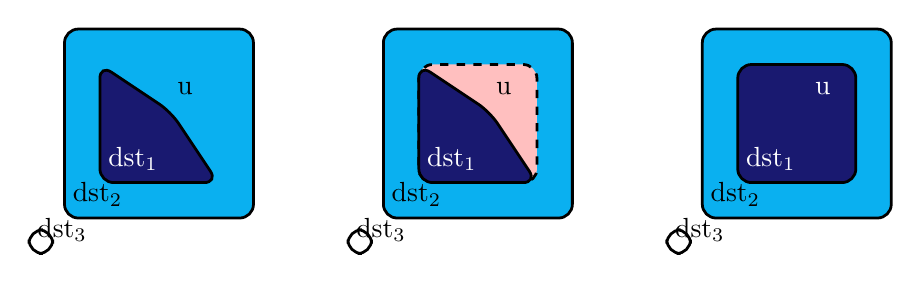
\begin{tikzpicture}[x=0.3cm, y=0.3cm,
      popped/.style={rounded corners=5pt, line width=1pt, draw, fill=MidnightBlue},
      fringe/.style={rounded corners=5pt, line width=1pt, draw, fill=ProcessBlue},
      popping/.style={rounded corners=5pt, line width=1pt, draw, dashed, fill=pink},
      unseen/.style={rounded corners=5pt, line width=1pt, draw}]
    \draw[unseen] (0,0) -- (\s,0) -- (\s,\s) -- (0,\s) -- cycle;
    \draw[fringe] (1.5,1.5) -- (9.5,1.5) -- (9.5,9.5) -- (1.5,9.5) -- cycle;
    \draw[popped] (3,3) -- (8,3) -- (6,6) -- (3,8) -- cycle;
    \node at (1.4,1) {dst$_3$};
    \node at (2.9,2.5) {dst$_2$};
    \node at (4.4,4) {\color{white}dst$_1$};
    \node at (6.6,7) {u};
    \tikzset{shift={(13.5,0)}}

    \draw[unseen] (0,0) -- (\s,0) -- (\s,\s) -- (0,\s) -- cycle;
    \draw[fringe] (1.5,1.5) -- (9.5,1.5) -- (9.5,9.5) -- (1.5,9.5) -- cycle;
    \draw[popping] (3,3) -- (8,3) -- (8,8) -- (3,8) -- cycle;
    \draw[popped] (3,3) -- (8,3) -- (6,6) -- (3,8) -- cycle;
    \node at (1.4,1) {dst$_3$};
    \node at (2.9,2.5) {dst$_2$};
    \node at (4.4,4) {\color{white}dst$_1$};
    \node at (6.6,7) {u};

    \tikzset{shift={(13.5,0)}}

    \draw[unseen] (0,0) -- (\s,0) -- (\s,\s) -- (0,\s) -- cycle;
    \draw[fringe] (1.5,1.5) -- (9.5,1.5) -- (9.5,9.5) -- (1.5,9.5) -- cycle;
    \draw[popped] (3,3) -- (8,3) -- (8,8) -- (3,8) -- cycle;
    \node at (1.4,1) {dst$_3$};
    \node at (2.9,2.5) {dst$_2$};
    \node at (4.4,4) {\color{white}dst$_1$};
    \node at (6.6,7) {\color{white}u};
  \end{tikzpicture}
  \caption{Popping $\m{u}$}
\end{figure}

Next, we must account for the ripple effect that popping
$\m{u}$ could have had on the other vertices.
In particular, it is possible that a vertex obeying $\m{inv\_unpopped}$ can
improve its cost via $\m{u}$, and that an unreachable vertex
obeying $\m{inv\_unseen}$ can now be reached via $\m{u}$.
The for loop repairs these breakages by
checking if a path via $\m{u}$ is an improvement for such vertices, and, if so,
edits both arrays and the priority queue as seen on line~\ref{code:update}.

The for loop's invariant is similar to that of the while loop---$\m{inv\_unseen}$
and $\m{inv\_popped}$ are preserved as-is, modulo the popping of
$\m{u}$ as discussed above. The key edit is in $\m{inv\_unpopped}$. blah blah blah

}



\begin{figure}[t]

\begin{lstlisting}[mathescape=true,showlines=true]
void dijkstra (int **g, int src, int *dist,
               int *prev, int size, int inf {
$\color{OliveGreen}//~\braces{\p{AdjMat}(\texttt{g},\gamma) *
\mathsf{array}(\texttt{dist}, \_) * \mathsf{array}(\texttt{prev}, \_)}$
 Item* temp = (Item*) mallocN(sizeof(Item));
 int* keys = mallocN (size * sizeof (int));
 PQ* pq = pq_make(size); int i, j, u, cost;
 for (i = 0; i < size; i++)
 { dist[i] = inf; prev[i] = inf; keys[i] = pq_push(pq,inf,i); } $\label{code:assigninf}$
 dist[src]= 0; prev[src]= src; pq_edit_priority(pq,keys[src],0);
 while (pq_size(pq) > 0) {
$\color{OliveGreen}//~\braces{{\color{red}\exists \m{dist}, \m{prev}, \m{popped}, \m{heap}}.~\p{AdjMat}(\texttt{g},\gamma) * {\color{red}\p{PQ}(\texttt{pq},\m{heap})} *
{\color{red}\mathsf{Item}(\texttt{temp}, \_)} * \null \\
\mathsf{array}(\texttt{dist},{\color{red}\m{dist}}) *
\mathsf{array}(\texttt{prev}, {\color{red}\m{prev}}) *
{\color{red}\mathsf{array}(\texttt{keys}, \m{keys}}) /| \null \\
{\color{red}\m{linked\_correctly}(\gamma, \m{heap}, \m{keys}, \m{dist}, \m{popped})} /| \null \\
{\color{red}\m{dijk\_correct}(\gamma,\texttt{src},\m{popped},\m{prev},\m{dist})}}$ $\label{code:whileinv}$
  pq_pop(pq, temp); u = temp->data; $\label{code:pop}$
  for (i = 0; i < size; i++) {
$\color{OliveGreen}//~\braces{{\color{red}\exists \m{dist'}, \m{prev'}, \m{heap'}}.~\p{AdjMat}(\texttt{g},\gamma) * \p{PQ}(\texttt{pq},{\color{red}\m{heap'}}) * \null \\
\mathsf{array}(\texttt{dist},\m{\color{red}dist'}) *
\mathsf{array}(\texttt{prev}, \m{\color{red}prev'}) *
\mathsf{array}(\texttt{keys}, \m{keys}) * \null \\
\mathsf{Item}(\texttt{temp}, \m{\color{red}(\texttt{keys[u]}, \texttt{dist[u]}, \texttt{u})}) /|
\m{\color{red}min(\texttt{dist[u]}, \m{heap'})} /| \null \\
{\m{linked\_correctly}(\gamma, \m{\color{red}heap'}, \m{keys}, \m{\color{red}dist'},
{\color{red}\m{popped} \uplus \{\texttt{u}\}})} /| \null \\
{\color{red}\m{dijk\_correct\_weak}({\color{OliveGreen}\gamma, \texttt{src}}, \m{popped} \uplus \{\texttt{u}\}, \m{prev'}, \m{dist'}, \texttt{i}, \texttt{u})}}$ $\label{code:forinv}$
   cost = getCell(g, u, i); $\label{code:cost}$
   if (cost < inf) {
    if (dist[i] > dist[u] + cost) { $\label{code:overflow}$
     dist[i] = dist[u] + cost; prev[i] = u; $\label{code:update1}$
     pq_edit_priority(pq, keys[i], dist[i]); $\label{code:update2}$
  }}}} $\color{OliveGreen}//~\braces{{\color{red}\exists \m{dist''}, \m{prev''}}.~\p{AdjMat}(\texttt{g},\gamma) * \p{PQ}(\texttt{pq},\m{\color{red}\emptyset}) * {\mathsf{Item}(\texttt{temp}, {\color{red}\_})} * \null \\
 \mathsf{array}(\texttt{dist},\m{\color{red}dist''}) *
 \mathsf{array}(\texttt{prev}, \m{\color{red}prev''}) *
 \mathsf{array}(\texttt{keys}, \m{keys}) /| \null \\
{\color{red}\forall \m{dst}.~0 \le \m{dst} < \texttt{size} -> \m{inv\_popped}}(\gamma, \m{src}, {\color{red}\m{\gamma.V}, \m{prev''}, \m{dist''}, \m{dst}})}$ $\label{code:end}$
 freeN (temp); pq_free (pq); freeN (keys); return; }
\end{lstlisting}
\vspace{-1em}
\caption{C code and proof sketch for Dijkstra's Algorithm.}
\vspace{-1em}
\label{fig:decorated}
\end{figure}



\hide{
$\color{OliveGreen}//~\braces{{\color{red}\exists \m{dist''}, \m{prev''},\m{heap''}}.~\p{AdjMat}(\texttt{g},\gamma) * \p{PQ}(\texttt{pq},\m{\color{red}heap''}) *
  \mathsf{array}(\texttt{dist},\m{\color{red}dist''}) * \null \\
  \mathsf{array}(\texttt{prev}, \m{\color{red}prev''}) *
  \mathsf{array}(\texttt{keys}, \m{keys}) *
  \mathsf{Item}(\texttt{temp}, \m{(\texttt{keys[u]}, \texttt{dist[u]}, \texttt{u})} /| \null \\
  \m{min(\texttt{dist[u]}, \m{heap'})} /|
  {\color{red}\m{heap''} = \m{heap'} [\texttt{keys[i]} \mapsto (\texttt{dist[i]},\texttt{i})]} /| \null \\
  {\m{\color{red}dijk\_correct}(\gamma, \texttt{src}, \m{popped'}, \m{\color{red}prev''}, \m{\color{red}dist''})}}$ $\label{code:caughtup}$
}



\section{Verified Dijkstra}
\label{sec:verification}


\begin{equation*}
\begin{split}
\p{list\_rep}(\gamma, \m{i}) &\defeq \texttt{data\_at  array  graph2mat}(\gamma)[\m{i}] \texttt{  list\_addr}(\gamma, \m{i}) \\
\vspace{1em}
\p{graph\_rep}(\gamma) &\defeq \underset{\texttt{vvalid}(\gamma,\m{v})}{\bigstar} \m{v}  \mapsto\p{list\_rep}(\gamma, \m{v})
\end{split}
\end{equation*}

\begin{equation*}
\begin{split}
&\!\!\!\!\!\!\m{path\_correct}(\gamma, \m{src}, \m{prev}, \m{dist}, \m{mom}, \m{p}) \; \defeq \; 
\m{valid\_path}(\gamma, \m{p}) /| \m{path\_ends}(\gamma, \m{p}, \m{src}, \m{dst}) /| \null \\
&\m{path\_cost}(\gamma, \m{p}) \not= \texttt{INF} /| \m{dist}[\m{dst}] = \m{path\_cost}(\gamma, \m{p}) /| \forall \m{a, b}.~\m(a,b) \in p -> \m{prev}[\m{b}] = \m{a} \\
\vspace{2em}
&\!\!\!\!\!\!\m{path\_globally\_optimal}(\gamma, \m{src}, \m{dst}, \m{p}) \; \defeq \; 
\forall \m{p'}.~\m{valid\_path}(\gamma, \m{p'}) -> \m{path\_ends}(\gamma, \m{p'}, \m{src}, \m{dst}) -> \\
&\hspace{20em}\m{path\_cost}(\gamma, \m{p}) \le \m{path\_cost}(\gamma, \m{p'}) \\
&\!\!\!\!\!\!\m{all\_hops\_in\_popped}(\m{p}, \m{priq}) \; \defeq \; 
\forall \m{a, b}.~\m{(a, b)} \in \m{p} -> \m{a} \in \m{popped}(\m{priq}) /| \m{b} \in \m{popped}(\m{priq})\\
&\!\!\!\!\!\!\m{all\_hops\_in\_popped\_weak}(\m{p}, \m{priq}, \texttt{u}) \; \defeq \; 
\forall \m{a, b}.~\m{(a, b)} \in \m{p} -> \m{a} \in \m{popped}(\m{priq}) /| \null \\ 
&\hspace{20em}\m{b} \in \m{popped}(\m{priq}) /| \m{a} \not= \texttt{u} /| \m{b} \not= \texttt{u} \\
\vspace{4em}
&\!\!\!\!\!\!\m{dijk\_correct}(\gamma, \m{src}, \m{prev}, \m{dist}, \m{priq}) \; \defeq \; \\
&\forall \m{dst}.~\texttt{0} \le \m{dst} < \texttt{SIZE} -> \m{inv\_popped}(\gamma, \m{src}, \m{prev}, \m{dist}, \m{priq}, \m{dst}) /| \null \\
&\hspace{11em}\m{inv\_unpopped}(\gamma, \m{src}, \m{prev}, \m{dist}, \m{priq}, \m{dst}) /| \null \\
&\hspace{11em}\m{inv\_unseen}(\gamma, \m{prev}, \m{dist}, \m{priq}, \m{dst}) \\
\vspace{1em}
&\!\!\!\!\!\!\m{dijk\_correct\_weak}(\gamma, \m{src}, \m{prev}, \m{dist}, \m{priq}, \texttt{i}, \texttt{u}, \texttt{SIZE}) \; \defeq \; \\
&\forall \m{dst}.~\texttt{0} \le \m{dst} < \texttt{SIZE} -> \m{inv\_popped}(\gamma, \m{src}, \m{prev}, \m{dist}, \m{priq}, \m{dst}) /| \null \\
&\hspace{11em}\m{inv\_unseen}(\gamma, \m{prev}, \m{dist}, \m{priq}, \m{dst}) /| \null \\
&\forall \m{dst}.~\texttt{0} \le \m{dst} < \texttt{i} -> \m{inv\_unpopped}(\gamma, \m{src}, \m{prev}, \m{dist}, \m{priq}, \m{dst}) /| \null \\
&\forall \m{dst}.~\texttt{i} \le \m{dst} < \texttt{SIZE} -> \m{inv\_unpopped\_weak}(\gamma, \m{src}, \m{prev}, \m{dist}, \m{priq}, \m{dst}, \texttt{u}) \\
\vspace{1em}
&\!\!\!\!\!\!\m{inv\_popped}(\gamma, \m{src}, \m{prev}, \m{dist}, \m{priq}, \m{dst}) \; \defeq \; \m{dst} \in \m{popped}(\m{priq}) -> \\
&\exists \m{p2dst}.~\m{path\_correct}(\gamma, \m{src}, \m{prev}, \m{dist}, \m{dst}, \m{p2dst}) /| \null \\
&\m{all\_hops\_in\_popped}(\m{p2dst}, \m{priq}) /|
\m{path\_globally\_optimal}(\gamma, \m{src}, \m{dst}, \m{p2dst}) \\
\vspace{1em}
&\!\!\!\!\!\!\m{inv\_unpopped}(\gamma, \m{src}, \m{prev}, \m{dist}, \m{priq}, \m{dst}) \; \defeq \; \m{priq}[\m{dst}] < \texttt{INF} -> \\
&\texttt{let } \m{mom} \texttt{ := } \m{prev}[\m{dst}] \texttt{ in } \exists \m{p2mom}.~\m{path\_correct}(\gamma, \m{src}, \m{prev}, \m{dist}, \m{mom}, \m{p2mom}) /| \null \\
&\m{all\_hops\_in\_popped}(\m{p2mom}, \m{priq}) /| \m{path\_globally\_optimal}(\gamma, \m{src}, \m{mom}, \m{p2mom}) /| \null \\
&\forall \m{mom', p2mom'}.~~\m{path\_correct}(\gamma, \m{src}, \m{prev}, \m{dist}, \m{mom'}, \m{p2mom'}) -> \\
&\m{all\_hops\_in\_popped}(\m{p2mom'}, \m{priq}) -> 
\m{path\_globally\_optimal}(\gamma, \m{src}, \m{mom'}, \m{p2mom'}) -> \\
&\m{path\_cost}(\m{p2mom} + \m{(mom, dst)}) \le \m{path\_cost}(\m{p2mom'} + \m{(mom', dst)}) \\
\vspace{1em}
&\!\!\!\!\!\!\m{inv\_unpopped\_weak}(\gamma, \m{src}, \m{prev}, \m{dist}, \m{priq}, \m{dst}) \; \defeq \; \m{priq}[\m{dst}] < \texttt{INF} -> \\
&\texttt{let } \m{mom} \texttt{ := } \m{prev}[\m{dst}] \texttt{ in } \exists \m{p2mom}.~\m{path\_correct}(\gamma, \m{src}, \m{prev}, \m{dist}, \m{mom}, \m{p2mom}) /| \null \\
&\m{all\_hops\_in\_popped\_weak}(\m{p2mom}, \m{priq}) /| \m{path\_globally\_optimal}(\gamma, \m{src}, \m{mom}, \m{p2mom}) /| \null \\
&\forall \m{mom', p2mom'}.~~\m{path\_correct}(\gamma, \m{src}, \m{prev}, \m{dist}, \m{mom'}, \m{p2mom'}) -> \\
&\m{all\_hops\_in\_popped\_weak}(\m{p2mom'}, \m{priq}) -> 
\m{path\_globally\_optimal}(\gamma, \m{src}, \m{mom'}, \m{p2mom'}) -> \\
&\m{path\_cost}(\m{p2mom} + \m{(mom, dst)}) \le \m{path\_cost}(\m{p2mom'} + \m{(mom', dst)}) \\
\vspace{1em}
&\!\!\!\!\!\!\m{inv\_unseen}(\gamma, \m{prev}, \m{dist}, \m{priq}, \m{dst}) \; \defeq \; \m{priq}[\m{dst}] = \texttt{INF} ->
(\m{dist}[\m{dst}] = \texttt{INF} /| \m{prev}[\m{dst}] = \texttt{INF})
\end{split}  
\end{equation*}

\section{Overflow Strikes Again}
\label{sec:overflow}
Dijkstra's algorithm clearly cannot work when a path
cost is greater than \texttt{INT\_MAX}.  A reasonable-looking restriction 
is to bound edge costs by 
$\left\lfloor\frac{\texttt{INT\_MAX}}{\texttt{size}-1}\right\rfloor$, since 
the longest optimal path has $\texttt{size}-1$ links and so the 
most expensive possible path costs no more than \texttt{INT\_MAX}.  
However, this has two flaws.  First, since we are writing real code in~C, 
rather than pseudocode in an idealized setting, we must reserve some 
concrete \texttt{int} value \texttt{inf} for ``infinity'', which has 
the special semantics that, if the best-known distance to a vertex~\m{x}
is \texttt{inf}, then~\m{x} is as-yet unreachable. 
A consequence of this is that reachable destination vertices cannot have a 
path cost of \texttt{inf}: if they did, this would be logged in the 
\m{dist} array and create an unpleasant ambiguity. 
Second, even though the best-known distances start at \texttt{inf} 
(see line~\ref{code:assigninf}) and only ever decrease from there, the code can 
overflow on lines~\ref{code:overflow}~and~\ref{code:update1}.

\begin{figure}[t]
\centering
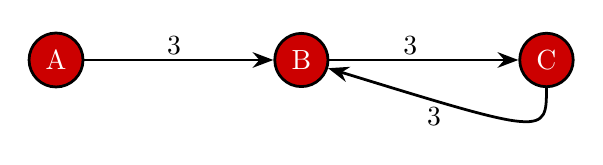
\begin{tikzpicture}[x=0.3cm, y=0.3cm,
  vert/.style={circle, line width=1pt, draw, fill=red}]
  \node[vert] (A) at (0,0) {\color{white}A};
  \node[vert] (B) [right = 8 of A] {\color{white}B};
  \node[vert] (C) [right = 8 of B] {\color{white}C};
  \draw [->,line width=1pt,arrows={-Stealth}] (A) -- (B);
  \draw [->,line width=1pt,arrows={-Stealth}] (B) -- (C);
  \draw [->,line width=1pt,arrows={-Stealth}] (C.south) .. controls ++(0, -2) .. (B);
  \node at (5,0.6) {3};
  \node at (15,0.6) {3};
  \node at (16,-2.4) {3};
\end{tikzpicture}
\caption{A graph that will result in overflow on a 3-bit machine.}
\label{fig:overflow}
\end{figure}

Consider applying Dijkstra's algorithm on a hypothetical 3-bit unsigned machine to 
the graph in figure~\ref{fig:overflow}.  The \texttt{size} of the graph is 3 nodes, and so the na\"ive edge-weight upper bound is $\left\lfloor\frac{\texttt{INT\_MAX}}{\texttt{size}-1}\right\rfloor = \left\lfloor\frac{7}{3-1}\right\rfloor = 3$, exactly as pictured in figure~\ref{fig:overflow}.  Indeed, a glance at the diagram is enough to tell that the true distance from the source~A~to vertices~B~and~C~are~3~and~6 respectively---both of which are representable with 3 bits, and so na\"ively all seems well.  %Unfortunately, Dijkstra's algorithm does not exactly work like that.  
Indeed, after processing vertices~A~and~B, 3~and~6~\emph{are} the costs reflected in the \m{dist} array for~B~and~C respectively---\emph{but unfortunately vertex~C~is still in the priority queue}.  After vertex~C~is popped on line~\ref{code:pop}, we fetch its neighbors in the \texttt{for} loop; vertex~B's cost of~3~is fetched on line~\ref{code:cost}.  On line~\ref{code:overflow} the currently optimal cost of~B~(3) is compared against the sum of the optimal cost of~C~(6) plus the just-retrieved cost of the edge from~C~to~B~(3).  Since $6+3$ overflows in 3-bit arithmetic, the comparison is not between~3~and~9 but in fact between~3~and~1!  Thus the code decides that a new cheaper path from~A~to~B~exists (in particular, A$\leadsto$B$\leadsto$C$\leadsto$B) and then trashes the \texttt{dist} and \texttt{prev} arrays on line~\ref{code:update1}.  %

Our code uses signed \texttt{int} rather than \texttt{unsigned int} so we have undefined behavior rather than defined-but-wrong behavior, but the essence of the overflow is identical.
Our solution is twofold.  First, we restrict the maximum edge cost to $\left\lfloor\frac{\texttt{INT\_MAX}}{\texttt{size+1}}\right\rfloor$, which in the 3-bit setting just described forces an edge cost of no more than~2.  Second, we require in the precondition that 
$\left\lfloor \frac{\texttt{INT\_MAX}}{\texttt{size}} \right\rfloor < \texttt{inf} \le \texttt{INT\_MAX} - \left\lfloor \frac{\texttt{INT\_MAX}}{\texttt{size}+1} \right\rfloor$, which in the 3-bit setting is 5.  Consider modifying figure~\ref{fig:overflow} to
have edge weights of~2~rather than~3.  After processing vertices~A~and~B, the distances to~B~and~C are no more than~2~and~4 respectively.  When we process vertex~C, the comparison on line~\ref{code:overflow} is thus between the previous best cost to~B~(2) and the candidate best cost to~B~via~C~(6); there is no overflow and the code behaves as advertised.



%% If you have bibdatabase file and want bibtex to generate the
%% bibitems, please use
%%
%\bibliographystyle{plainurl}% the mandatory bibstyle

\bibliographystyle{splncs04}
\bibliography{dijkstra}

%% The Appendices part is started with the command \appendix;
%% appendix sections are then done as normal sections
\appendix
% 
\appendix

{\color{magenta}
\section{Simplifying ramification entailments}
After applying \infrulestyle{Solve Ramify-PQ}, it is often desirable to break the ramification entailment into smaller disjoint pieces before trying to solve it directly.
One common case is to ``frame out'' an unneeded part of the global state:
\[
\infrule{Frame Ramify-Q}
{G_1 \vdash L_1 * \forall x.~ (L_2 --* G_2)}  
{G_1 * F \vdash L_1 * \forall x.~ \big(L_2 --* (G_2 * F)\big) }
{\begin{array}{c}F \text{ ignores} \\ \MV(c) \cup \{x\} \end{array}} \qquad \qquad \qquad
\]
In fact \infrulestyle{Frame Ramify-Q} is a consequence of the more general \[
\infrule{Split Ramify-Q}
{G_1 \vdash L_1 * \big(\forall x.~ (L_2 --* G_2)\big) \! \! \! \! \\
 G_1' \vdash L_1' * \big(\forall x.~ (L_2' --* G_2')\big) }
{G_1 * G_1' \vdash L_1 * L_1' * \Big(\forall x.~ \big((L_2 * L_2') --* (G_2 * G_2')\big)\Big)} {}
\]
In general the strategy is to apply \infrulestyle{Frame Ramify-P} and \infrulestyle{Split Ramify-P} until the ramification entailments are as small as they can be (while remaining true!) before using \infrulestyle{Solve Ramify-P} on the remaining ``atoms''.

The situation is unfortunately a little messier when the postconditions contain existential quantifiers.

\[\text{UNSOUND-RAM-Q-SPLIT}\]
\Rule{}
{G_1 \vdash L_1 * (\exists x, L_1' (x) --* \exists x, G_1'(x)) \\
G_2 \vdash L_2 * (\exists x, L_2' (x) --* \exists x, G_2'(x)) \\}
{G_1 * G_2 \vdash L_1 * L_2 * (\exists x, L_1'(x) * L_2'(x) --* \exists x, G_1'(x) * G_2'(x)) }


\[
\infrule{Ramify-Q}
{\{ L \} ~ c ~ \{\exists x.~ L' \} \\
 G \vdash L * \big(\forall x.~ (L' --* G')\big)}
{\{ G \} ~ c ~ \{ \exists x.~G' \}}{}
\]

}


\section{Junk}
{\color{magenta} Universally-quantified metavariables can appear free in the predicates to make further connections.
Assuming that the abstracted pre- and postconditions $A$, $B$, $C$, and $D$ above all use \li{x}, we proceed
as follows.  First we introduce a new fresh metavariable $x$ whose value will be equal to \li{x} after the localization, and then choose $F \stackrel{\Delta}{=} [\li{x} |-> x] (C -* D)$, that is we substitute the program
variable \li{x} for the metavariable $x$.  Since we have substituted away \li{x}, $F$ ignores it and so we satisfy the side condition on \infrulestyle{Solve Ramify-P}.  We then must strengthen $C$ into $C' \stackrel{\Delta}{=} C /| \li{x} = x$ to make the connection at the appropriate program point.  Now we are left with the entailments
\[
\begin{array}{lcl}
\li{x} = 5 /| A & |- & (\li{x} = 5 /| B) * F \\
F & |- & (\li{x} = 6 /| C') -* (x = 6 /| D)
\end{array}
\]
To further relate the earlier and later values of \li{x} in $F$ we can introduce a second fresh $x'$ and use $B' \stackrel{\Delta}{=} B /| \li{x} = x'$.
}

The \infrulestyle{Ramify} rule is sound but interacts poorly with modified program variables (as in lines~\ref{code:markbeforetripleramify}--\ref{code:markaftertripleramify} of Figure~\ref{fig:markgraph}) {\color{magenta} and
localized existentials (as in lines~\ref{code:beforemarkl}--\ref{code:aftermarkl})}.  Both of these limitations are annoying enough in paper proofs and graduate to major headaches in mechanized ones.  Happily, we show how to overcome both limitations in \S\ref{sec:freevars} and \S\ref{sec:existentials}, respectively, by presenting new variants of \infrulestyle{Ramify}.  Our notation carries over without significant change: just use the new rules to enable the more general ramification entailments they permit.
%When in doubt the most general rule, \infrulestyle{Ramify-PQ} from \S\ref{sec:existentials}, implies all of the others.

\section{More junk}
\hide{
\section{Ramification Rules}


\Rule{Frame  }
{\{ P \} c \{Q \} \\
  F \text{ is stable w.r.t. } \MV(c)\\}
 {\{P * F \} c \{ Q * F \}}

\Rule{Ramification   }
{\{ L \} c \{L' \} \\
 G \vdash L * (L' -* G') \\
 (L' -* G') \text{ is stable w.r.t. } \MV(c)\\}
{\{ G \} c \{ G' \}}

\Rule{Ramification-P }
{\{ L \} c \{L' \} \\
 G \vdash L * \Box^{\llbracket c \rrbracket} (L' -* G') \\}
{\{ G \} c \{ G' \}}

\subsection{P for Pure Facts}

Separation logic has been mechanized by many projects CITE CITE CITE.
In many of them, like VST and Charge!, expressing the value of a local
variable (a variable stored in stack) is a pure fact rather than a
spatial fact. Because the side condition of ramification rule requires $(L' -* G')$ to be stable w.r.t. modified local variables in $c$\footnote{In previous papers, the side conditions of Frame rule and ramification rule are usually expressed as ``$\FV(F) \cap \MV(c) = \emptyset$'' and ``$\FV(L' -* G') \cap \MV(c) = \emptyset$''. The side conditions used in this paper are equivalent with typical ones if the semantic interpretation of $\FV$ is used. All the previous mentioned projects takes semantic interpretation instead of syntactical interpretation.}, it is almost impossible to apply ramification rule in any practical situations in these systems. In this paper, we present a pure-facts-related rule (we call it ramification-P rule, or just P rule, in the rest of this paper) such that it is sound and practical in the most general setting of separation logics.

The primary ramification rule is essentially an application of the frame rule using $(L' -* G')$ as frame.
Thus, the key point of handling pure facts is to find a legal frame even if $(L' -* G')$ is not stable w.r.t. $\MV(c)$. This frame is $\Box^{\llbracket c \rrbracket} (L' -* G')$ in ramification-P rule.
\begin{eqnarray*}
m \models \Box^R P &  \Leftrightarrow  & \forall m', \text{ if } m\xrightarrow{R}m' \text{ then } m' \models P \\
m \xrightarrow{\llbracket c \rrbracket} m' & \Leftrightarrow &   \text{$m$ and $m'$ coincide everywhere} \\
&& \text{except $\MV(c)$} \\
P \text{ is stable} &  \Leftrightarrow  & \forall m \ m',  \text{if $m$ and $m'$ coincide everywhere} \\
\text{w.r.t. $S$} && \text{except $S$, then $m \models P$ iff $m' \models P$}
\end{eqnarray*}

Here, $\Box$ represents the necessity modal operator. The formula $\Box^{\llbracket c \rrbracket} (L' -* G')$ says, it is true on a state $m$ if and only if for any state $m'$, if $m$ and $m'$
coincide everywhere except on the variables modified by $c$, then $(L' -* G')$ is true on $m'$.

Based on the combination frame rule, consequence rule and three basic facts below, we can immediate prove ramification-P rule.
\begin{quotation}
(a) $\Box^{\llbracket c \rrbracket} (L' -* G')$ is stable w.r.t. $\MV(c).$\footnote{This can be proved directly from the definition of $\llbracket c \rrbracket$ and stability, and the fact that $\llbracket c \rrbracket$ is an equivalence relation.}

(b) $G \vdash L * \Box^{\llbracket c \rrbracket} (L' -* G')$. (Assumption)

(c) $L' *  \Box^{\llbracket c \rrbracket} (L' -* G') \vdash G'$. \footnote{When $R$ is reflexive, T-Axiom of modal logic is sound, i.e. for any $P$, $\Box^R P \vdash P$. As $\llbracket c \rrbracket$ is reflexive, we know the fact that $\Box^{\llbracket c \rrbracket} (L' -* G') \vdash L' -* G'$, which is immediate followed by $L' *  \Box^{\llbracket c \rrbracket (L' -* G')} \vdash G'$.}
\end{quotation}

\subsection{Establish the Assumption Entailment of P Rule}

It is well-known that the proof theory with magic wand is already complicated, so generally speaking, it will not be a easy task to prove an entailment with magic wand together with modality. However, people need to prove an entailment with form
\begin{equation}G \vdash  L * \Box^R (L' -* G') \label{eqn:Passu} \end{equation}
at first when applying ramification-P rule. Luckily, this special form makes the task simpler.

First of all, SOLVE-RAM-P rule can turn the proof goal into two wand-free and modality-free entailments. Specifically, people only need to find an $R$-stable predicate $F$, such that $G \vdash L * F$ and $F * L' \vdash G'$ are both true.

SOLVE-RAM-P alone is not a satisfactory proof theory because in that case using P rule would have no different from using frame rule directly. The key point here is that, an entailment with form \ref{Passu} can be proved in a modularized way. For primary ramification rule, CITE proposed two proof rule, RAM-FRAME and RAM-SPLIT\footnote{\Rule{RAM-FRAME }
{G \vdash L * (L' -* G') \\
F \text{ is stable w.r.t. } \MV(c) \\}
{G * F \vdash L * (L' -* G' * F) }

\Rule{RAM-SPLIT }
{G_1 \vdash L_1 * (L_1' -* G_1') \\
G_2 \vdash L_2 * (L_2' -* G_2') \\}
{G_1 * G_2 \vdash L_1 * L_2 * (L_1' * L_2' -* G_1' * G_2') }
}, to divide an entailment with form $G \vdash L * (L' -* G')$ into small pieces. When it comes to ramification-P rule, two corresponding proof rules, RAM-P-FRAME and RAM-P-SPLIT are still sound.

\Rule{SOLVE-RAM-P }
{G \vdash L * F\\
F * L' \vdash G' \\
F \text{ is stable w.r.t. } \MV(c) \\}
{G \vdash L * \Box^{\llbracket c \rrbracket} (L' -* G') }

\Rule{RAM-P-FRAME }
{G \vdash L * \Box^{\llbracket c \rrbracket} (L' -* G') \\
F \text{ is stable w.r.t. } \MV(c) \\}
{G * F \vdash L * \Box^{\llbracket c \rrbracket} (L' -* G' * F) }

\Rule{RAM-P-SPLIT }
{G_1 \vdash L_1 * \Box^{\llbracket c \rrbracket} (L_1' -* G_1') \\
G_2 \vdash L_2 * \Box^{\llbracket c \rrbracket} (L_2' -* G_2') \\}
{G_1 * G_2 \vdash L_1 * L_2 * \Box^{\llbracket c \rrbracket} (L_1' * L_2' -* G_1' * G_2') }

To conclude, if $L'$ and $G'$ are two separating conjunctions of a bunch of atomic predicates, RAM-P-FRAME and RAM-P-SPLIT can establish \ref{Passu} from entailments with the same form but smaller size. Atomic sized entailments can be proved using SOLVE-RAM-P. They are usually general purposed entailments and do not need to be proved for every single program. In section \ref{vst}, we will see examples of this approach for real programs.

\subsection{Q for Quantifiers}

In secion ???, we have already seen that it is a practical approach writing pre/postconditions as a separating conjunction of a list of atomic predicates (which makes RAM-P-FRAME and RAM-P-SPLIT useful). But unfortunately, an existential in post condition (also very common as we have seen in section ???) will prevent us from using these two rules. Now, one natural solution is to find other proof rules, like the following one, to deal with existential quantifiers.
\[\text{UNSOUND-RAM-Q-SPLIT}\]
\Rule{}
{G_1 \vdash L_1 * (\exists x, L_1' (x) -* \exists x, G_1'(x)) \\
G_2 \vdash L_2 * (\exists x, L_2' (x) -* \exists x, G_2'(x)) \\}
{G_1 * G_2 \vdash L_1 * L_2 * (\exists x, L_1'(x) * L_2'(x) -* \exists x, G_1'(x) * G_2'(x)) }

But this rule is NOT sound (even though we have not add $\Box$ operator to deal with local variable related stuff). The reason is that, given the local piece of memory satisfies $L_1'(x) * L_2'(x)$ for some specific $x$, we know that it can be split into two small piece of memory and they satisfies $L_1'(x)$ and $L_2'(x)$ respectively. Then the assumption tell us that the global piece can be split into two corresponding piece, $G_1'(x_1)$ and $G_2'(x_2)$ are true on them for some specific $x_1$ and $x_2$. Now the problem comes. Only if we could prove $x_1 = x_2$, we could prove the conclusion. But we cannot.

The key point of the failure above is that the frame, $\exists x, L' (x) -* \exists x, G'(x)$, says if $L'(x)$ is true on local then there is another (might be same one) $x_0$ such that $G'(x_0)$ is true on global. This is too weak for modularity. In many practical cases, we can in fact prove that $G'(x)$ should be true for the exact same $x$. This observation brings us to the ramification-PQ rule here.
\Rule{Ramification-PQ}
{\{ L \} c \{ \exists x, L' (x) \} \\
 G \vdash L * \Box^{\llbracket c \rrbracket} (\forall x, L' (x) -* G' (x)) \\}
{\{ G \} c \{ \exists x, G' (x)\}}

PQ rule can be directly derived from P rule by using the following theorem from separation logic\footnote{
$$\frac{\frac{\frac{\forall x, (L' (x) -* G' (x)) \vdash L' (x_0) -* G' (x_0)}{\forall x, (L' (x) -* G' (x)) * L' (x_0) \vdash G' (x_0)}}
{\forall x, (L' (x) -* G' (x)) * \exists x, L' (x) \vdash \exists x, G' (x)}}
{\forall x, (L' (x) -* G' (x)) \vdash \exists x, L' (x) -* \exists x, G' (x)}$$
}.
$$\forall x, (L' (x) -* G' (x)) \vdash \exists x, L' (x) -* \exists x, G' (x)$$
Like what we do to P rule, three corresponding rules, SOLVE-RAM-PQ, RAM-PQ-FRAME and RAM-PQ-SPLIT, are proved sound and can be used to establish the assumption of PQ rule in a modularized way. For those who do not care about local variable related issue, a ramification-Q rule can be used to deal with existentials. For the sake for space here, we omit them in this paper.

\subsection{Ramification in Decorated Programs}

One nice thing about Hoare logic is that it enables people to write combinational proofs. Moreover, such kind of proofs can be written in a nice printed form, decorated programs. %For example,
% \begin{figure}[h]
%\begin{tabular}{c | c}
%\begin{lstlisting}
%$\{\ \ \ P_1 \ \ \ \}$
%  c1;
%$\{\ \ \ P_2 \ \ \ \}$
%$\{\ \ \ P_3 \ \ \ \}$
%  c2;
%$\{\ \ \ P_4 \ \ \ \}$
%$\{\ \ \ P_5 \ \ \ \}$
%\end{lstlisting}
%&
%$$
%\inference[]
%{\triple{P_1}{c1}{P_2} &
%\inference[]
%{P_2 \vdash P_3 \\ P_4 \vdash P_5 \\ \triple{P_3}{c2}{P_4} }
%{\triple{P_2}{c2}{P_5}}
%}
%{\triple{P_1}{c1;c2}{P_5}}
%$$
% \\
%%TODO: fix format
%\end{tabular}
%\end{figure}

%The decorated program on the left is actually representing the Hoare logic proof on the right side.
By adding a new pattern, we call it localized and unlocalize, ramification proofs can also be presented in a decorated programs.

\begin{figure}[h]
\begin{tabular}{c | c}
\begin{lstlisting}
$\{\ \ \ G_1 \ \ \ \}$
$\searrow \{\ \ \ L_1 \ \ \ \}$
      c1;
      ...
      c5;
$\swarrow \{\ \ \ L_2 \ \ \ \}$
$\{\ \ \ G_2 \ \ \ \}$
\end{lstlisting}
&
$$
\inference[]
{\triple{L_1}{c1;...;c5}{L_2} \\
G_1 \vdash L_1 * (L_2 -* G_2)
}
{\triple{G_1}{c1;...;c5}{G_2}}
$$
 \\
%TODO: fix format
\end{tabular}
\caption{Localize and unlocalize in decorated programs}
\label{figure:lul}
\end{figure}

Figure \ref{figure:lul} shows such a decorated program. We call the action in line 2 \emph{localize} and call the action in line 6 \emph{unlocalize}. A Hoare logic proof using ramification rule can always be written as a decorated program with localize and unlocalize, as long as wherever we write do unlocalize action, we should prove a side condition, e.g. $G_1 \vdash L_1 * (L_2 -* G_2)$ in this example.
}

\section{Remaining proof of \infrulestyle{Ramify-PQ}}
\label{apx}

See figure \ref{fig:remainrampq}.

\begin{figure*}[t]
\[
\infrule{}
{
  L_1 |- L_1 \\
  \infrule{}
  {
    \infrule{}
    {
      \infrule{}
      {
        \infrule{}
        {
          \infrule{}
          {
            \infrule{}
            {
              \infrule{}
              {
                \infrule{}
                {
                  \infrule{}
                  {
                    \infrule{}
                    {
                      [x |-> x_0] (L_2 -* G_2) |- [x |-> x_0](L_2 -* G_2)
                    } {
                      \forall x.~ (L_2 -* G_2) |- [x |-> x_0](L_2 -* G_2)
                    } {\forall \mathsf{e}}
                  } {
                    \forall x.~ (L_2 -* G_2) |- ([x |-> x_0]L_2) -* ([x |-> x_0]G_2)
                  } {\textrm{substitute}}
                } {
                  \big(\forall x.~ (L_2 -* G_2)\big) * [x |-> x_0]L_2 |- [x |-> x_0]G_2
                } {(3)}
              } {
                \big(\forall x.~ (L_2 -* G_2)\big) * [x |-> x_0]L_2 |- \exists x.~ G_2
              } {\exists \mathsf{i}}
            } {
            \big(\forall x.~ (L_2 -* G_2)\big) * (\exists x.~ L_2) |- \exists x.~ G_2
            } {\exists \mathsf{e}}
          } {
            \forall x.~ (L_2 -* G_2) |- (\exists x.~ L_2) -* (\exists x.~ G_2)
          } {(3)}
        } {
          |- \big(\forall x.~ (L_2 -* G_2)\big) => \big((\exists x.~ L_2) -* (\exists x.~ G_2)\big)
        } {=> \mathsf{i}}
      } {
        |- \pguards{c}\Big(\big(\forall x.~ (L_2 -* G_2)\big) => \big((\exists x.~ L_2) -* (\exists x.~ G_2)\big)\Big)
      } {\mathsf{N}}
    } {
      |- \Big(\pguards{c}\big(\forall x.~ (L_2 -* G_2)\big) \Big) => \Big( \pguards{c}\big((\exists x.~ L_2) -* (\exists x.~ G_2)\big) \Big)
    } {\mathsf{K}}
  } {
    \pguards{c}\big(\forall x.~ (L_2 -* G_2)\big) |- \pguards{c}\big((\exists x.~ L_2) -* (\exists x.~ G_2)\big)
  } {\mathsf{i} =>}
} {
  L_1 * \pguards{c}\big(\forall x.~ (L_2 -* G_2)\big) |- L_1 * \pguards{c}\big((\exists x.~ L_2) -* (\exists x.~ G_2)\big)
} {* \textrm{ split} }
\]
\caption{Remaining proof of \infrulestyle{Ramify-PQ}}
\label{fig:remainrampq}
\end{figure*}

\subsection{More junk}
 precision helps enable the forward style
of reasoning used by HIP/SLEEK.  To use $\mu_{\mathsf{A}}$, our graph predicate
would have $\rhd$, \emph{i.e.}

%forall w w1 w2 : A, P w1 -> P w2 -> join_sub w1 w -> join_sub w2 w -> w1 = w2

$\rhd P$ is not , for any $P$.

  We do not believe
that this point has been observed before in the literature.  Precision is a standard technical
property that separation logic predicates can have

. Informally, a contractive
function is one such that if $\tau$ is approximately equal to
$\sigma$, then $F_p(\tau)$ is more accurately equal to
$F_p(\sigma)$.


  whose
mechanically verified its soundness. People can still define recursive
predicate $P$ through $F_p$ and $\mu_{\mathsf{R}}$, but this time the
$F_p$ needs to be

 The approximate equality is achieved by a data type as
a sequence of accurate approximations taken successively. This idea is
called step-indexing.

We attempted to formulate $\mathtt{graph}$ through fixed-point
functions $\mu_{\mathsf{T}}$ and $\mu_{\mathsf{R}}$. The contractive
functor $\mathtt{graphF}$ is defined as follows:
\[\label{eqn:graphFcotr}
  \begin{split}
  & \mathtt{graphF}(Q, x, \gamma)\defeq (x = 0 \wedge \mathtt{emp})
    \vee \\ & \exists d,l,r . \gamma(x)=(d,l,r) \wedge x \mapsto
    d,l,r\, \ocon \triangleright Q(l, \gamma) \ocon \triangleright
    Q(r, \gamma)
  \end{split}
\]
where $\triangleright$ is is the ``later'' operator which implements
the machinery of step-indexing. Note that $\mathtt{graphF}$ is a
normal predicate without recursion. $\mathtt{graph}$ is defined as
$\mu_{\mathsf{R}}\,\mathtt{graphF}$. One advantage of this definition
of $\mathtt{graph}$ is that proof by induction is possible because the
step-index can be seen as the inductive number. Unfortunately
$\mathtt{graph}$ is not \emph{precise} under this definition. For any
spatial predicate $P$, $\text{precise}(P)$ means whenever $P$ is
satisfied on a sub-state, that sub-state must be unique. Being precise
is a crucial requirement of $\mathtt{graph}$ for key theorems in our
framework. Further-more, it can be proved that for any predicate $P$,
$\triangleright P$ is not precise. So this defintion is abandoned.

Similarly we can define a covariant functor $\mathtt{graphQ}$ as
follows:
\[\label{eqn:graphFco}
  \begin{split}
  & \mathtt{graphQ}(Q, x, \gamma)\defeq (x = 0 \wedge
  \mathtt{emp}) \vee \\ & \exists d,l,r . \gamma(x)=(d,l,r) \wedge  x
  \mapsto d,l,r\, \ocon Q(l, \gamma) \ocon Q(r, \gamma)
  \end{split}
\]
The only difference between $\mathtt{graphQ}$ and $\mathtt{graphF}$ is
that $\mathtt{graphQ}$ does not have the $\triangleright$
operator. With this definition $\mathtt{graph}$ can be defined as
$\mu_{\mathsf{T}}\,\mathtt{graphQ}$. Again we need to prove the
preciseness of $\mathtt{graph}$. Since there is no induction principle
for this definition, we tried to prove it through the following lemma:
\begin{equation}\label{eqn:graph_iter}
\mathtt{graph}(x, \gamma) \dashv\vdash
\underset{v\in\mathit{reach}(\gamma, x)}{\bigstar} v\mapsto\gamma(v)
\end{equation}
where $\mathit{reach}(\gamma, x)$ is the set of nodes reachable from
$x$ in $\gamma$ and 




\begin{figure*}
  \begin{lstlisting}
struct Node {
    int m;
    struct Node * l;
    struct Node * r; };

// We use $R$ to represent $\p{reachable}(\gamma,\tx x)$

void spanning(struct Node * x) { // $\{\p{graph}(\tx{x},\gamma)/|\gamma(\tx{x}).1=0\}$
    struct Node * l, * r; int root_mark;
// $\{\p{graph}(\tx x,\gamma) /| \exists l,r.~ \gamma(\tx{x}) = (0,l,r)\}$
// $\{\p{graph}(\tx x,\gamma) /| \gamma(\tx{x}) = (0,l,r)\}$
// $\{\p{vertices\_at}(\p{reachable}(\gamma,\tx x), \gamma) /| \gamma(\tx{x}) = (0,l,r)\}$
// $\{\p{vertices\_at}(R, \gamma) /| \gamma(\tx{x}) = (0,l,r)\}$
// $\searrow \{\tx x|-> 0,l,r /| \gamma(\tx{x}) = (0,l,r)\}$
    l = x -> l;
    r = x -> r;
    x -> m = 1;
// $\swarrow \{\tx x|-> 1,\tx{l},\tx{r} /| \gamma(\tx{x}) = (0,\tx{l},\tx{r}) /| \exists \gamma_1.~ \m{mark1}(\gamma, \tx{x}, \gamma_1)\}$
// $\{\exists \gamma_1.~\p{vertices\_at}(R, \gamma_1) /| \gamma(\tx{x}) = (0,\tx{l},\tx{r}) /| \m{mark1}(\gamma, \tx{x}, \gamma_1)\}$
// $\{\p{vertices\_at}(R, \gamma_1) /| \gamma(\tx{x}) = (0,\tx{l},\tx{r}) /| \m{mark1}(\gamma, \tx{x}, \gamma_1)\}$
    if (l) {
//   $\{\p{vertices\_at}(R, \gamma_1) /| \gamma(\tx{x}) = (0,\tx{l},\tx{r}) /| \exists m_2, l_2, r_2.~\gamma_1(\tx{l})=(m_2, l_2, r_2) /| \m{mark1}(\gamma, \tx{x}, \gamma_1)\}$
//   $\{\p{vertices\_at}(R, \gamma_1) /| \gamma(\tx{x}) = (0,\tx{l},\tx{r}) /| \gamma_1(\tx{l})=(m_2, l_2, r_2) /| \m{mark1}(\gamma, \tx{x}, \gamma_1)\}$
//   $\searrow\{\tx{l} |-> m_2, -, l_2, r_2\}$
        root_mark = l -> m;
//   $\swarrow\{\tx{l} |-> m_2, -, l_2, r_2/|m_2 = \tx{root\_mark}\}$
//   $\{\p{vertices\_at}(R, \gamma_1)/| \gamma(\tx{x}) = (0,\tx{l},\tx{r})/|\gamma_1(\tx{l})=(m_2, l_2, r_2)/|m_2 = \tx{root\_mark} /| \m{mark1}(\gamma, \tx{x}, \gamma_1)\}$
        if (root_mark == 0) {
//     $\{\p{vertices\_at}(R, \gamma_1)/|\gamma(\tx{x}) = (0,\tx{l},\tx{r})/|\gamma_1(\tx{l})=(0, l_2, r_2) /| \m{mark1}(\gamma, \tx{x}, \gamma_1)\}$
//     $\searrow\{\p{graph}(\tx{l}, \gamma_1)/|\gamma_1(\tx{l})=(0, l_2, r_2)\}$
            spanning(l);
//     $\swarrow\{\exists \gamma_2. ~\p{vertices\_at}(\p{reachable}(\gamma_1,\tx l), \gamma_2)/|\gamma_1(\tx{l})=(0, l_2, r_2)/|\m{span}(\gamma_1,\tx{l},\gamma_2)\}$
//     $\{\exists \gamma_2. ~\p{vertices\_at}(R, \gamma_2)/|\gamma(\tx{x}) = (0,\tx{l},\tx{r}) /|\gamma_1(\tx{l})=(0, l_2, r_2) /| \m{mark1}(\gamma, \tx{x}, \gamma_1) /|\m{span}(\gamma_1,\tx{l},\gamma_2)\}$
        } else {
//     $\{\p{vertices\_at}(R, \gamma_1)/| \gamma(\tx{x}) = (0,\tx{l},\tx{r})/|\gamma_1(\tx{l})=(1, l_2, r_2)  /| \m{mark1}(\gamma, \tx{x}, \gamma_1)\}$
//     $\searrow \{\tx x|-> 0,\tx{l},\tx{r} /| \gamma(\tx{x}) = (0,\tx{l},\tx{r})\}$
            x -> l = 0;
//     $\swarrow \{\tx x|-> 0,0,\tx{r} /| \gamma(\tx{x}) = (0,\tx{l},\tx{r})\}$
//     $\{\exists \gamma_2. ~\p{vertices\_at}(R, \gamma_2)/|\gamma(\tx{x}) = (0,\tx{l},\tx{r})/|\gamma_1(\tx{l})=(1, l_2, r_2) /| \m{mark1}(\gamma, \tx{x}, \gamma_1) /| \m{e\_rm}(\gamma_1, \tx{x}.\text{L}, \gamma_2)\}$
        }
//   $\{\exists\gamma_2.~\p{vertices\_at}(R,\gamma_2)/| \gamma(\tx{x}) = (0,\tx{l},\tx{r})  /| \m{mark1}(\gamma, \tx{x}, \gamma_1) /| \m{e\_span}(\gamma_1,\tx{x}.\text{L},\gamma_2)\}$
    }
    else {
//   $\{\p{vertices\_at}(R, \gamma_1) /| \gamma(\tx{x}) = (0,\tx{l},\tx{r}) /| \tx{l}= 0  /| \m{mark1}(\gamma, \tx{x}, \gamma_1)\}$
        skip;
//   $\{\exists\gamma_2. ~\p{vertices\_at}(R,\gamma_2)/| \gamma(\tx{x}) = (0,\tx{l},\tx{r})  /| \m{mark1}(\gamma, \tx{x}, \gamma_1) /| \m{e\_span}(\gamma_1,\tx{x}.\text{L},\gamma_2)\}$
    }
// $\{\exists\gamma_2. ~\p{vertices\_at}(R,\gamma_2)/| \gamma(\tx{x}) = (0,\tx{l},\tx{r})  /| \m{mark1}(\gamma, \tx{x}, \gamma_1) /| \m{e\_span}(\gamma_1,\tx{x}.\text{L},\gamma_2)\}$
// $\{\p{vertices\_at}(R,\gamma_2)/| \gamma(\tx{x}) = (0,\tx{l},\tx{r})  /| \m{mark1}(\gamma, \tx{x}, \gamma_1) /|  \m{e\_span}(\gamma_1,\tx{x}.\text{L},\gamma_2)\}$
    if (r) {
//   $\{\p{vertices\_at}(R, \gamma_2) /| \gamma(\tx{x}) = (0,\tx{l},\tx{r}) /| \exists m_2, l_2, r_2.~\gamma_1(\tx{l})=(m_2, l_2, r_2) /| \m{mark1}(\gamma, \tx{x}, \gamma_1)/| \m{e\_span}(\gamma_1,\tx{x}.\text{L},\gamma_2)\}$
//   $\{\p{vertices\_at}(R, \gamma_2) /| \gamma(\tx{x}) = (0,\tx{l},\tx{r}) /| \gamma_2(\tx{r})=(m_2, l_2, r_2) /| \m{mark1}(\gamma, \tx{x}, \gamma_1)/| \m{e\_span}(\gamma_1,\tx{x}.\text{L},\gamma_2)\}$
//   $\searrow\{\tx{r} |-> m_2, -, l_2, r_2\}$
        root_mark = r -> m;
//   $\swarrow\{\tx{r} |-> m_2, -, l_2, r_2/|m_2 = \tx{root\_mark}\}$
//   $\{\p{vertices\_at}(R, \gamma_2)/| \gamma(\tx{x}) = (0,\tx{l},\tx{r})/|\gamma_2(\tx{r})=(m_2, l_2, r_2)/|m_2 = \tx{root\_mark} /| \m{mark1}(\gamma, \tx{x}, \gamma_1)/| \m{e\_span}(\gamma_1,\tx{x}.\text{L},\gamma_2)\}$
        if (root_mark == 0) {
//     $\{\p{vertices\_at}(R, \gamma_2)/|\gamma(\tx{x}) = (0,\tx{l},\tx{r})/|\gamma_2(\tx{r})=(0, l_2, r_2) /| \m{mark1}(\gamma, \tx{x}, \gamma_1)/| \m{e\_span}(\gamma_1,\tx{x}.\text{L},\gamma_2)\}$
//     $\searrow\{\p{graph}(\tx{r}, \gamma_2)/|\gamma_2(\tx{r})=(0, l_2, r_2)\}$
           spanning(r);
//     $\swarrow\{\exists \gamma_3. ~\p{vertices\_at}(\p{reachable}(\gamma_2,\tx r), \gamma_3)/|\gamma_2(\tx{r})=(0, l_2, r_2)/|\m{span}(\gamma_2,\tx{r},\gamma_3)\}$
//     $\{\exists \gamma_3. ~\p{vertices\_at}(R, \gamma_3)/|\gamma(\tx{x}) = (0,\tx{l},\tx{r}) /|\gamma_2(\tx{r})=(0, l_2, r_2) /| \m{mark1}(\gamma, \tx{x}, \gamma_1) /|\m{span}(\gamma_1,\tx{l},\gamma_2)/|\m{span}(\gamma_2,\tx{r},\gamma_3)\}$
        } else {
//     $\{\p{vertices\_at}(R, \gamma_2)/| \gamma(\tx{x}) = (0,\tx{l},\tx{r})/|\gamma_2(\tx{r})=(1, l_2, r_2)  /| \m{mark1}(\gamma, \tx{x}, \gamma_1) /| \m{e\_span}(\gamma_1,\tx{x}.\text{L},\gamma_2)\}$
//     $\searrow \{\tx x|-> 0,?l,\tx{r} /| \gamma(\tx{x}) = (0,?l,\tx{r})\}$
            x -> r = 0;
//     $\swarrow \{\tx x|-> 0,?l,\tx{r} /| \gamma(\tx{x}) = (0,?l,\tx{r})\}$
//     $\{\exists \gamma_3. ~\p{vertices\_at}(R, \gamma_3)/|\gamma(\tx{x}) = (0,\tx{l},\tx{r})/|\gamma_2(\tx{r})=(1, l_2, r_2) /| \m{mark1}(\gamma, \tx{x}, \gamma_1) /| \m{e\_span}(\gamma_1,\tx{x}.\text{L},\gamma_2) /| \m{e\_rm}(\gamma_2, \tx{x}.\text{R}, \gamma_3)\}$
        }
//   $\{\exists\gamma_3.~\p{vertices\_at}(R,\gamma_3)/| \gamma(\tx{x}) = (0,\tx{l},\tx{r})  /| \m{mark1}(\gamma, \tx{x}, \gamma_1) /| \m{e\_span}(\gamma_1,\tx{x}.\text{L},\gamma_2) /| \m{e\_span}(\gamma_2,\tx{x}.\text{R},\gamma_3)\}$
    }
    else {
//   $\{\p{vertices\_at}(R, \gamma_2) /| \gamma(\tx{x}) = (0,\tx{l},\tx{r}) /| \tx{r}= 0  /| \m{mark1}(\gamma, \tx{x}, \gamma_1)  /| \m{e\_span}(\gamma_1,\tx{x}.\text{L},\gamma_2)\}$
        skip;
//   $\{\exists\gamma_3.~\p{vertices\_at}(R,\gamma_3)/| \gamma(\tx{x}) = (0,\tx{l},\tx{r})  /| \m{mark1}(\gamma, \tx{x}, \gamma_1) /| \m{e\_span}(\gamma_1,\tx{x}.\text{L},\gamma_2) /| \m{e\_span}(\gamma_2,\tx{x}.\text{R},\gamma_3)\}$
    }
//   $\{\exists\gamma_3.~\p{vertices\_at}(R,\gamma_3)/| \gamma(\tx{x}) = (0,\tx{l},\tx{r})  /| \m{mark1}(\gamma, \tx{x}, \gamma_1) /| \m{e\_span}(\gamma_1,\tx{x}.\text{L},\gamma_2) /| \m{e\_span}(\gamma_2,\tx{x}.\text{R},\gamma_3)\}$
} // $\{\exists \gamma_3.~\p{vertex\_at}(\p{reachable}(\gamma, \tx{x}), \gamma_3)/|\m{span}(\gamma,\tx{x},\gamma_3)\}$
\end{lstlisting}

\caption{Clight code and proof sketch for bigraph spanning tree.}
\label{fig:spanning-full}

\end{figure*}


%%\end{thebibliography}
\end{document}
\endinput
%%

	
	\section{Verified Prim in C}
	\label{sec:prim}
	Here we discuss our verifications of the classic MST algorithms Prim and Kruskal.  Although our machine-checked proofs are about real~C~code, in this section we take a higher-level approach than we did in \S\ref{sec:dijkstra}, focusing on our key algorithmic findings and overall experience.  Accordingly, we only provide pseudocode for Prim's algorithm rather than a decorated program and do not show any code for Kruskal's.  Our development contains our~C~code and formal proofs~\cite{anonrepo}.

\subsection{Prim's Algorithm}
\label{sec:prim}

\vspace{-3.5em}
\begin{figure}
\[
\begin{array}{@{}l@{~~}|@{~~}l@{}}
\begin{minipage}{0.475\textwidth}
\begin{lstlisting}
MST-PRIM(G,w,r):
 for each u in G.V
  u.key = INF
  u.parent = NIL $\hide{code:primsetinitparent}$
 r.key = 0 $\label{code:primsetroot}$
 Q = G.V
 while Q $\neq$ $\emptyset$
  u = EXTRACT-MIN(Q) $\hide{code:primextractmin}$
  for each v in G.Adj[u]
   if v $\in$ Q and w(u,v) $<$ v.key
    v.parent = u
    v.key = w(u,v) $\hide{code:primeditpri}$
\end{lstlisting} \end{minipage} &
\begin{minipage}{0.5\textwidth}
\begin{lstlisting}[numbers=none]
MST-NOROOT-PRIM(G,w):
 for each u in G.V
  u.key = INF
  u.parent = NIL

 Q = G.V
 while Q $\neq$ $\emptyset$
  u = EXTRACT-MIN(Q)
  for each v in G.Adj[u]
   if v $\in$ Q and w(u,v) $<$ v.key
    v.parent = u
    v.key = w(u,v)
\end{lstlisting}
\end{minipage}
\end{array}
\]
\caption{Left: Prim's algorithm from CLRS~\cite{clrs}. Right: the same omitting line 5.}
\label{fig:prims}
\end{figure}

\vspace{-1.5em}
We put the pseudocode for Prim's algorithm in figure~\ref{fig:prims}; the code on the left-hand side is directly from CLRS, whereas the code on the right omits line 5 and will be discussed in~\S\ref{sec:primforest}.  Note that lines~5 and~12 contain implicit calls to the PQ's \texttt{edit\_priority}.  Since the pseudocode only compares \texttt{key}s (\emph{i.e.}, edge weights) rather than doing arithmetic on them \emph{\`a la} Dijkstra, there are no potential overflows and it is reasonable to set \texttt{INF} to \texttt{INT\_MAX} in~C.

Indeed, our initial verifications of~C~code were largely ``turning the crank'' once we had the definitions and associated lemma support for pure/abstract undirected graphs, trees, \emph{etc.} discussed in \S\ref{sec:newundirected}.  Accordingly, from an engineering perspective, our initial contribution was a demonstration that this new graph machinery was sufficient to verify real code.  \note{We also demonstrated that our pure reasoning was isolated from our spatial reasoning by verifying three versions of~C~code with slightly different memory layouts for adjacency matrices with the same pure theorems (our proof base for these versions differs by less than 1\%, exactly for the portion of the~C~code that accesses the graph representation in memory)}.  By reusing much pure and spatial reasoning that had been originally developed for our verification of Dijkstra, we also demonstrated that our extensions to CertiGraph from~\S\ref{sec:extensions} were generic rather than verification-specific.

\subsection{Prim's Algorithm handles multiple components out of the box}
\label{sec:primforest}

Textbook discussions of Prim's algorithm are usually limited to single-component input graphs (\emph{a.k.a.} connected graphs), producing a minimum spanning tree.  It is widely believed that Prim's is not directly applicable to graphs with multiple components, which should produce a minimum spanning forest.  For example, both Rozen~\cite{rozen} and Sedgewick~\cite{sedgewick} leave the extension to multiple components as an formal exercise for the reader, whereas Kepner and Gilbert suggest that multiple-component graphs should be handled by first finding the components and then running Prim on each component~\cite{kepnergilbert}.  This appears to be the standard solution, appearing in numerous lectures and implementations\footnote{Another standard solution is to use Kruskal's \hide{or Boruvka's~\cite{boruuvka1926jistem}} algorithm instead.}. %CLRS does not mention the case of disconnected graphs

After we completed our initial verification, a close examination of our formal invariants showed us that the algorithm \emph{exactly as given by standard textbooks} will properly handle multi-component graphs \textit{in a single run}.  \note{The key is that in a fully connected graph, any vertex $\texttt{u}$ removed from the PQ on line~8 must have $\texttt{u.key} < \texttt{INF}$, \emph{i.e.} must be immediately reachable from the spanning tree that is in the process of being built.}  However, nothing in the code itself relies upon this connectedness fact!  All we need is that $\texttt{u}$ is the ``closest vertex'' to the ``current component,'' assuming one exists.  If $\texttt{u.key}=\texttt{INF}$ \emph{and} \texttt{u} is a minimum of the PQ, then it simply means that the ``previous component'' is done, and we have started spanning tree construction on a new unconnected component ``rooted'' at \texttt{u}, yielding a forest.  The node $\texttt{u}$'s parent will remain \texttt{NIL}, at it was after the setup loop on line~4, indicating that it is the root of a spanning tree.  Its \texttt{key} will be $\texttt{INF}$ rather than $0$, but the \texttt{key}s are \emph{internal to Prim's algorithm}: clients only get back the spanning forest as encoded in the \texttt{parent} pointers\footnote{The \texttt{key}s simply record the edge-weight connecting a vertex to its candidate parent; recall that line~12 is really a call to the PQ's \texttt{edit\_priority}.  If a client wishes to know this edge weight, it can simply look up the edge in the graph.}.

Having made this discovery, we updated our proofs to support the new weaker precondition, which is what we currently formally verify in Coq~\cite{Coq}.
A little further thought led to the realization that since Prim can handle arbitrary numbers of components, the initialization of the root's \texttt{key} in line~5 is in fact unnecessary.  Accordingly, if we remove this line and the associated function argument \texttt{r} from \texttt{MST-PRIM} (\emph{i.e.} the code on the right half of figure~\ref{fig:prims}), the algorithm still works correctly.  Moreover, \emph{the program invariants become simpler} because we no longer need to treat a specified vertex (\texttt{r}) in a distinguished manner.  Our formal development verifies this version of the algorithm as well~\cite{anonrepo}.

\subsection{Related work on Prim in algorithms and formal methods}
\label{sec:relworkprim}

Prim's algorithm was in fact first developed by the Czech mathematician Vojt\v{e}ch Jarn\'{i}k in 1930~\cite{prim1:jarnik} before being rediscovered by Robert Prim in 1957~\cite{prim2:prim} and a third time by Edsger~W.~Dijkstra in 1959~\cite{prim3:dijkstra}.  Both Prim's and Dijkstra's treatment explicitly assumes a connected graph; although we cannot read Czech, some time with Google translate suggests that Jarn\'{i}k's treatment probably does the same.  Most modern textbook treatment (\emph{e.g.} \cite{kepnergilbert,sedgewick,rozen,DBLP:books/daglib/0022194,clrs}) seems to derive from either Prim's or Dijkstra's treatment.
More casual references such as Wikipedia~\cite{prim:wiki} and innumerable lecture slides are presumably derived from the textbooks cited.  We have not found any references that state that Prim's algorithm \emph{without modification} applies to multi-component graphs, even when executable code is provided: \emph{e.g.}, Heineman \emph{et al.} provide C++ code that aligns closely with our C code~\cite{heineman2008algorithms}, but do not mention that their code works equally well on multi-component graphs.  Indeed, many sources promulgate the false proposition that modifications to the algorithm are necessary to handle multi-component graphs (\emph{e.g.},~\cite{kepnergilbert,sedgewick,rozen,prim:wiki}).  Likewise, we have found no reference that removes the initialization step (line~5) in figure~\ref{fig:prims}) from the standard algorithm.

Prim's algorithm has been the focus of a few previous formalization efforts.  Guttman formalised and proved the correctness of Prim's algorithm using Stone-Kleene relation algebras in Isabelle/HOL~\cite{DBLP:conf/ictac/Guttmann16}.  He works in an idealized formal environment that does not require the development of explicit data structures; his code does not appear to be executable.  Lammich \emph{et al.} provided a verification of Prim's algorithm~\cite{DBLP:journals/afp/LammichN19}.  Lammich \emph{et al.} also work within the idealized formal environment of Isabelle/HOL, but in contrast to Guttman develop efficient purely functional data structures and extract them to executable code.  Both Guttman and Lammich explicitly require that the input graph be connected. % and produce a tree.

%axiomatizes  
%his second paper that their earlier proof of Prim's assumed "".



%  We make two immediate observations on CLRS's pseudocode: first, that they do not give an explicit definition for

% Note that  does not explicitly define \texttt{EXTRACT-MIN}

%are often limited to the case where the input graph is a connected graph. This is reasonable, as their purpose is to teach the concept of minimum-spanning \textit{tree} algorithms. However, they seldom expand on the subject of spanning forests for disconnected graphs. For example, . \textit{Discrete Mathematics and Its Applications} leaves it as an exercise to the reader, while \textit{Graph Algorithms in the Language of Linear Algebra}~\cite{kepnergilbert} suggests running Prim's on each component of the disconnected graph to obtain a minimum spanning forest. The last appears to be the most common solution, with suggesting this.


\hide{
\begin{figure}[H]
\begin{tikzpicture} [auto, node distance =2 cm and 2cm ,on grid, semithick, state/.style ={circle}]
\node[state] (V0) {$\m{v_0}$};
\node[state] (V1) [right=of V0] {$\m{v_1}$};
\node[state] (V2) [below=of V0] {$\m{v_2}$};
\node[state] (V3) [below right=of V0] {$\m{v_3}$};
\node[color=green] (V4) [right=of V3] {$\m{v_3}$};
\node[color=green] (V5) [right=of V4] {$\m{v_5}$};
\draw[color=red] (V0) edge [ultra thick] node[above=0.15 cm] {$5$} (V1);
\path (V0) edge node[left=0.15 cm] {$6$} (V2);
\path (V0) edge [thin] node[above right=0.05 cm] {$5$} (V3);
\path[color=red] (V1) edge [ultra thick] node[right=0.15 cm] {$5$} (V3);
\path[color=red] (V2) edge [ultra thick] node[below=0.15 cm] {$4$} (V3);
\path (V4) edge node[below=0.15 cm] {$1$} (V5);
\end{tikzpicture}
\caption{Figure of a partial Prim's execution with root $\m{v_0}$. A spanning tree for the left component has been found as indicated in red, while $\m{v_4}$ and $\m{v_5}$ are in the priority queue with weight \texttt{INF}. As our \texttt{EXTRACT-MIN} tolerates \texttt{INF}, our implementation will pop them from the priority queue and proceed as usual, instead of terminating with only the left tree.}
\end{figure}

From the above figure, we demonstrate that our simple priority queue will always pop vertices regardless of its weight. If the popped vertex has weight \texttt{INF}, its parent will also be at its default invalid value, indicating that no edge was added to the graph. We then continue the algorithm as usual, updating the weights of adjacent vertices. As a result, our Prim implementation can return a minimal spanning forest without ``premature termination".

Is our assumption that \texttt{EXTRACT-MIN} can pop \texttt{INF} weight vertices reasonable? We argue that it is, because the abstract algorithm in CLRS makes no statement about \texttt{INF} beyond the initialization. As the algorithm pushes the vertices into queue with weight \texttt{INF}, it is reasonable to say the priority queue can tolerate items with weight \texttt{INF}. Doing so simplifies \texttt{EXTRACT-MIN} to a \texttt{popMin} operation using the priority queue's API, without requiring additional lines of code to further check for specific weights.

Consequently, our code allows a simple implementation of Prim's to return a forest for a disconnected input graph, in a single run of the algorithm without needing to identify the disconnected components beforehand. It is important to note that we do not explicitly define ``components", nor do we tag \texttt{u} as a``new root". It is sufficient to prove that the loop invariant is satisfied whether \texttt{key[u]~< INF} or \texttt{key[u] = INF}.

Note that the priority queue used for this verification is still tied to \texttt{INF}, and thus in the verification our argument is weakened to ``\texttt{INF} is a valid weight in the priority queue" rather than ``membership in the priority queue is independent of \texttt{INF}". Work on a stronger priority queue which completely dissociates from \texttt{INF} was to be delivered by Aquinas Hobor since May 2020.
}

%  If they wish to determine the edge cost from a node to its parent, they can look it up in the graph, with the special case

%We observed that our code is able to return a minimum spanning forest when the input graph is disconnected, . The reason for this is: We treat a vertex of weight \texttt{INF} and a vertex's membership in the priority queue as \textit{separate} matters. A vertex can be in the priority queue with weight \texttt{INF}, represented by \texttt{key[u] = INF}, and this indicates that \texttt{u} is \textit{not} connected to any previously popped vertex; otherwise its weight would have been previously lowered. However, our priority queue does not care about its items having specific weights, only that the item it pops is always the one with the lowest weight. Thus, when a vertex \texttt{u} is returned, it is possible that \texttt{u} has weight \texttt{INF} - the scenario where all vertices remaining in the queue has weight \texttt{INF}, indicating all of them are disconnected from the current forest.

%Rather than start with a distinguished root vertex, we simply start with zero components, and the first vertex we extract (chosen arbitrarily by the PQ) becomes the root of the initial

%A further observation is that if we dissociate \texttt{INF} and the priority queue, then the input root required by Prim's is no longer necessary. The root's key is artificially set to 0 in Prim's, which kickstarts the main loop. However, since our emptiness check and \texttt{EXTRACT-MIN} implementation can return vertices with \texttt{INF} weight, the loop will start as long as there are un-popped vertices. Thus, we suggest it is possible to remove the \texttt{rt} parameter. Doing so simplifies the proof, because we do not have to reason about the artificially weighted \texttt{key[rt]}. The noroot-variant is in Figure 4 at the beginning of this section, while the verified implementation of Prim's without root is in \texttt{noroot\_prim.c}.

%They push their version of \texttt{INF} into the priority queue during the setup, and do not perform any explicit rejections of \texttt{INF}, simply popping from the priority queue at the \texttt{EXTRACT-MIN} step. However, they do not discuss minimum spanning forests, hence this observation is not recorded.

	
	\section{Verified Kruskal in C}
	\label{sec:kruskal}
	\texttt{MST-KRUSKAL}(\textit{G},\textit{w})
\newline
A = $\varnothing$
\newline
for each vertex \textit{v} $\in$ \textit{G.V}
\newline
$\hspace*{4mm}$ \texttt{MAKE-SET}(\textit{v})
\newline
sort the edges of \textit{G.E} into nonincreasing order by weight w
\newline
for each edge \textit{(u,v)} $\in$ \textit{G.E}, taken in nonicreasing order by weight
\newline
$\hspace*{4mm}$if \texttt{FIND-SET}(\textit{u}) $\neq$ \texttt{FIND-SET}(\textit{v})
\newline
$\hspace*{8mm}$\textit{A} = \textit{A} $\cup$ {\textit{(u,v)}}
\newline
$\hspace*{8mm}$\texttt{UNION}(\textit{u},\textit{v})
\newline
return \textit{A}
\begin{center}Abstract Kruskal's algorithm from CLRS~\cite{clrs}
\end{center}

\subsection{Edge list representation, multi-graph trimming, and subtle differences of graphs in different representations}
Kruskal's algorithm differs from Prim's and even Dijkstra's in that it directly operates on the edges of the input graph, rather than the latter two's vertex-based approaches. Consequently, in C implementations it is useful to pass the graph in as a list of graph edges, rather than an adjacency matrix or list. This also simplifies the sorting necessary in Kruskal's.
\newline\newline
We define a separate spatial representation of graphs as an edge list, and observe slight differences between the graphs that can be represented by an edge list and an adjacency-matrix representation. As mentioned in the Prim's section, in a symmetric adjacency matrix, $(u,v)$ and $(v,u)$ are considered the same edge; however, this is not true for an edge list, where a list can contain $(u,v)$ and $(v,u)$, even multiple copies of them. We do not prove the latter case for convenience reasons, but prove the former, to demonstrate the difference between an edge list representation and adjacency matrix representation.
\newline
\begin{lstlisting}
struct edge {
	int weight;
	int src;
	int dst;
};

struct graph {
	int V; //number of vertices {0...V-1}
	int E; //number of edges in the edgelist
	struct edge *edge_list;
};
//Consider a graph with edges {weight=1,src=0,dst=1}
//	and {weight=2,src=1,dst=0}
\end{lstlisting}
\begin{center}
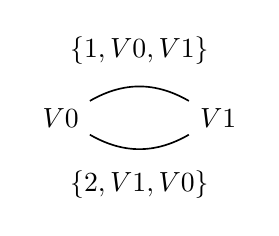
\begin{tikzpicture} [auto, node distance =2 cm and 2cm ,on grid, semithick, state/.style ={ circle}]
	\node[state] (V0) {$V0$};
	\node[state] (V1) [right=of V0] {$V1$};
	\path (V0) edge [bend left] node[above=0.15 cm] {$\{1,V0,V1\}$} (V1);
	\path (V1) edge [bend left] node[below=0.15 cm] {$\{2,V1,V0\}$} (V0);
\end{tikzpicture}
\end{center}
\begin{center}
Example of one kind of multi-graph representable by the above C edge-list implementation, which we have verified that Kruskal's algorithm is able to prune. We did not verify the case where another possible edge $\{2,V0,V1\}$ is in the edge list, for convenience
\end{center}

\subsection{Reusing previously verified union-find} %%why is there such an absurdly large space?
Kruskal's algorithm requires a union-find data structure to keep track of the state of connectedness in the graph. We made use of one of our previously verified union-find implementations. The union-find data structures were represented by their own specialized graph, denoted \texttt{UFGraph} within the kruskal verification.
\newline\newline
However, as the verified union-find implementations had no client using them until now, we discovered that the postconditions of using the union-find structures were difficult to use for Kruskal's verification. Kruskal's algorithm uses union-find to track the connectedness of vertices. However, the union-find implementations were verified prior to the introduction of such undirected graph properties, and thus were not designed with connectedness in mind. To that end, my research partner Anshuman has extended lemmas about the results of union and find operations as an analog to connectivity.
\newline\newline
We are pleased to say that no change was required for the existing union-find definitions, lemmas, specifications and verification. Instead, we proved that the postcondition of any of our union-find implementations, yields an analog to connectivity in undirected graphs. In other words, the verified postcondition was satisfactory, and just required translation into what we wanted in the context of Kruskal's.
\newline\newline
We mention this to emphasise the modularity and buildability of VST and CertiGraph infrastructure, that we were able to use previously, independently proven code in a bigger system later. The verification and internal details of the union-find system are furthermore independent from that of Kruskal's, whose proof only required the preconditions and postconditions of whichever union-find implementation we decided to use.

    \section{Verified binary heap}
    \label{sec:binheap}
    \lstset{style=myTinyStyle}

Binary heaps are a classic data structure for imperative programs~\cite{clrs,sedgewick}.  Briefly, binary heaps embed a heap-ordered tree in an array and use arithmetic on indices to navigate between a parent and its left and right children.  In addition to providing the standard \texttt{insert} and \texttt{remove-min}/\texttt{remove-max} operations (depending on whether it is a min- or max-ordered heap) in logarithmic time, binary heaps can by upgraded to support two nontrivial operations.  First, Floyd's \texttt{heapify} function builds a binary heap from an unordered array in linear time, and as a related upgrade, \texttt{heapsort} performs a worst-case linearithmic-time sort using only constant additional space.  Second, binary heaps can be upgraded to support logarithmic-time \texttt{decrease-} and \texttt{increase-priority} operations, which we generalize straightforwardly into \texttt{edit\_priority}.

Binary heaps are a good fit for our graph algorithms because Dijkstra's and Prim's algorithms need to edit priorities, and a constant-space \texttt{heapsort} is appropriate for the sparse edge-list-represented graphs typically targeted by Kruskal's.  The~C language has poor support for polymorphic higher-order functions, and a binary heap that supports \texttt{edit\_priority} is half as fast as a binary heap that does not.  Accordingly, we implement binary heaps in C three times:
\[
\begin{array}{l@{\quad}c@{\quad}c@{\quad}c@{\quad}l}
\text{Name} & \text{Heap order} & \texttt{edit\_priority} & \texttt{heapify} & \text{Payload} \\
\hline
\text{basic} & \text{min} & \text{no} & \text{yes} & \texttt{void*} \\
\text{advanced} & \text{min} & \text{yes} & \text{no} & \texttt{int} \\
\text{Kruskal} & \text{max} & \text{no} & \text{yes} & \texttt{int, int} \text{ (\emph{i.e.}, unboxed)}
\end{array}
\]
Priorities are of type \texttt{int}.  %\note[too much detail, too soon?]{The ``advanced'' implementation requires each item to be tagged to a ``key'', which is used to lookup the item whose priority must be changed; these keys are \texttt{unsigned int}s.}
The Kruskal-specific implementation is stripped down to the bare minimum required to implement \texttt{heapsort} (\emph{e.g.} it does not support \texttt{insert}).  We next overview these verifications in three parts: basic heap operations, \texttt{heapify} and \texttt{heapsort} operations, and the \texttt{edit\_priority} operation.

\subsection{The basic heap operations of insertion and min/max-removal}
\label{sec:heapinsertremove}

Because we are juggling three implementations, we take some care to factor our verification to maximize reuse.  First, each C implementation has its own exchange and comparison functions that handle the nitty-gritty of the payload and choose between a min or max heap.  The following lines are from the ``basic'' implementation, in which the ``payload'' (\texttt{data} field) is of type \texttt{void*}:
\begin{lstlisting}[firstnumber=5]
void exch(unsigned int j, unsigned int k, Item arr[]) {
 int priority = arr[j].priority; void* data = arr[j].data;
 arr[j].priority = arr[k].priority; arr[j].data = arr[k].data;
 arr[k].priority = priority; arr[k].data = data; }
int less(unsigned int j, unsigned int k, Item arr[]) {
 return (arr[j].priority <= arr[k].priority); }
\end{lstlisting}
These C functions are specified as refinements of Gallina functions that exchange polymorphic data in lists and compare objects in an abstract preordered set; we verify them in VST after a little irksome engineering.  The payoff is that the key heap operations, which, following Sedgewick~\cite{sedgewick}, we call \texttt{swim} and \texttt{sink}, can use identical~C code (up to alpha renaming) in all three implementations:
\begin{lstlisting}[firstnumber=last]
void swim(unsigned int k, Item arr[]) {
 while (k > ROOT_IDX && less (k, PARENT(k), arr)) {
  exch(k, PARENT(k), arr); k = PARENT(k);         } }
void sink (unsigned int k, Item arr[], unsigned int available) {
 while (LEFT_CHILD(k) < available) {
  unsigned j = LEFT_CHILD(k);
  if (j+1 < available && less(j+1, j, arr)) j++; $\label{code:sinkplusplus}$
  if (less(k, j, arr)) break; exch(k, j, arr); k = j;        } }
\end{lstlisting}
These functions involve a number of complexities, both at the algorithms level and at the semantics-of-C level.  At the C level, there is the potential for a rather subtle bug in the macros \texttt{ROOT\_IDX}, \texttt{PARENT}, etc.  Abstractly, these are simple: the root is in index 0; the children of $x$ at roughly $2x$ and the parent at roughly~$\frac{x}{2}$, with $\pm1$ as necessary.  The danger is thinking that because the variables are \texttt{unsigned int}, all arithmetic will occur in this domain; in fact we must force the associated constants into \texttt{unsigned int} as well:
\[
\begin{array}{@{}l@{~~}|@{~}l@{}}
\begin{minipage}{0.475\textwidth}
\begin{lstlisting}
#define ROOT_IDX  0u
#define PARENT(x) (x-1u)/2u
\end{lstlisting} \end{minipage} &
\begin{minipage}{0.5\textwidth}
\lstset{firstnumber=3}
\begin{lstlisting}
#define LEFT_CHILD(x)  (2u*x)+1u
#define RIGHT_CHILD(x) 2u*(x+1u)
\end{lstlisting}
\end{minipage}
\end{array}
\]
A second C-semantics issue is the potential for overflow within \texttt{LEFT\_CHILD} and \texttt{RIGHT\_CHILD} (as well as the increments on line~\ref{code:sinkplusplus}), and underflow within the \texttt{PARENT} macro (if \texttt{x} should ever be 0).  To avoid this overflow, the precondition of \texttt{sink} requires that when $\texttt{k}$ is in bounds (\emph{i.e.}, $\texttt{k} < \texttt{available}$), then $2\cdot(\texttt{available}-1) \leq \texttt{max\_unsigned}$.  An edge case occurs when deleting the last element from a heap ($\texttt{k}=\texttt{available}$); we then require $2\cdot\texttt{k}\leq \texttt{max\_unsigned}$.

\lstset{style=CoqStyle}

At the algorithmic level, both the \texttt{swim} and \texttt{sink} functions involve nontrivial loop invariants; \texttt{sink} is complicated by the further need to support Floyd's \texttt{heapify}, during which a large portion of the array is unordered.  Accordingly, we build Gallina models of both functions and show that they restore heap order given a mostly-ordered input heap.  There are two different versions of ``mostly-ordered''. Specifically, \texttt{swim} uses a ``bottom-up'' version:
\begin{lstlisting}[firstnumber=5]
Definition weak_heapOrdered2 (L : list A) (j : nat) : Prop :=
 ($\forall$ i b, i $\neq$ j $\rightarrow$ nth_error L i = Some b $\rightarrow$
   $\forall$ a, nth_error L (parent i) = Some a $\rightarrow$ a $\preceq$ b) $\wedge$
 (grandsOk L j root_idx).
\end{lstlisting}
whereas \texttt{sink} uses a ``top-down'' version:
\begin{lstlisting}[firstnumber=last]
Definition weak_heapOrdered_bounded (L:list A) (k:nat) (j:nat) :=
 ($\forall$ i a, i $\ge$ k $\rightarrow$ i $\neq$ j $\rightarrow$ nth_error L i = Some a $\rightarrow$
  ($\forall$ b, nth_error L (left_child i) = Some b $\rightarrow$ a $\preceq$ b) $\wedge$
  ($\forall$ c, nth_error L (right_child i) = Some c $\rightarrow$ a $\preceq$ c)) $\wedge$
 (grandsOk L j k).
\end{lstlisting}
The parameter \texttt{j} indicates a ``hole'', at which the heap may not be heap-ordered; \texttt{grandsOk} bridges this hole by
ordering the parent and the children of \texttt{j}:
\begin{lstlisting}
Definition grandsOk (L : list A) (j : nat) (k : nat) : Prop :=
  j $\neq$ root_idx $\rightarrow$ parent j $\geq$ k $\rightarrow$
    $\forall$ gs bb, parent gs = j $\rightarrow$ nth_error L gs = Some bb $\rightarrow$
      $\forall$ a, nth_error L (parent j) = Some a $\rightarrow$ a $\preceq$ bb.
\end{lstlisting}
The parameter \texttt{k} is used to support Floyd's \texttt{heapify}: it bounds the portion of the list in which elements are heap-ordered (with the exception of \texttt{j}).  The proofs that the Gallina \texttt{swim} and \texttt{sink} can restore (bounded) heap-orderedness involve a number of edge cases, but given the above definitions go through.  The invariants of the~C~versions of \texttt{swim} and \texttt{sink} are stated via the associated
Gallina versions, thereby delegating all heap-ordering proofs to the Gallina versions.

The insertion and remove functions we verify are in fact ``non-checking'' versions (\texttt{insert\_nc} and \texttt{remove\_nc}): their preconditions assume there is room in the heap to add or an item in the heap to remove.  In the context of Dijkstra and Prim, these preconditions can be proven to hold.  The associated verifications involve a little separation logic hackery (specifically, to \textsc{Frame} away the ``junk'' part of the heap-array from the ``live'' part), but are straightforward using VST.  We avoid the overflow issue in \texttt{sink} by bounding the maximum capacity of the heap: $4 \le 12\cdot\texttt{capacity} \leq \texttt{max\_unsigned}$; the magic number 12 comes from the size of the underlying data structure in~C.  We require users to prove this bound on heap creation, and thereafter handle it under the hood.

\lstset{style=myTinyStyle}

\subsection{Bottom-up heapify and heapsort}
\label{sec:heapsort}

Floyd's bottom-up procedure for constructing a binary heap in linear time, and using a binary heap to sort, are classics of the literature~\cite{clrs,sedgewick}.  Happily, while the asymptotic bound on heap construction is nontrivial, the implementations of both are basically repeated calls to \texttt{sink} (and exchanges to remove the root):
\begin{lstlisting}[firstnumber=19]
void build_heap(Item arr[], unsigned int size) {
 unsigned int start = PARENT(size); $\label{code:parentunderflow}$
 while(1) { sink(start, arr, size);
            if (start == 0) break; start--;  } }
void heapsort_rev(Item* arr, unsigned int size) {
 build_heap(arr,size); $\label{code:buildheapsort}$
 while (size > 1) { size--;
  exch(ROOT_IDX, size, arr); sink(ROOT_IDX, arr, size); } }
\end{lstlisting}
Given that in \S\ref{sec:heapinsertremove} we already generalized the specification for \texttt{sink} to handle a portion of the array being unordered, the verification of these functions is straightforward.  There is, however, the possibility of a subtle underflow on line~\ref{code:parentunderflow}, in the case when building an empty heap (\emph{i.e.}, $\texttt{size}=0$).  In turn, this means that \texttt{heapsort\_rev} as given above cannot sort empty lists; in our ``basic'' implementation we strengthen the precondition accordingly, whereas in our ``Kruskal'' implementation we add a line before~\ref{code:buildheapsort} that \texttt{return}s when $\texttt{size}=0$.  We use a max-heap for Kruskal because heapsort yields a \emph{reverse} sorted list.

\subsection{Modifying an element's priority}
\label{sec:modpri}

In contrast to \texttt{heapify} and \texttt{heapsort}, standard algorithms textbooks are vague on the implementation of \texttt{edit\_priority}~\cite{clrs,sedgewick}.  The idea is that, during \texttt{insert}, each item is associated not only with its usual \texttt{int} priority
but also a unique \texttt{unsigned int} ``key''.
This key is generated during \texttt{insert} and returned to the client.
Internally, the binary heap maintains a secondary array \texttt{key\_table} that maps each key to the current location of the associated item within the primary heap array. The client calls \texttt{edit\_priority} by supplying the key associated with the item
it wishes to modify, and the binary heap looks up the key in the \texttt{key\_table} to
locate the item in the heap array before calling \texttt{sink} or \texttt{swim}. To keep everything linked together, the \texttt{key\_table} is modified during \texttt{exch}ange.

One detail entirely missing from standard textbooks is how to generate the keys on insert.  The initial idea is to have a global counter starting at 0, which is then increased on each insert.  Unfortunately, this is unsound: during (very) long runs involving both \texttt{insert} and \texttt{remove-min}, this key counter will overflow.  Although overflow is defined in C for \texttt{unsigned int}, this overflow is fatal algorithmically: multiple items could be assigned the same key.

A better method is to store a key field within each heap-item in the main array.  These keys are initialized to $0..(\texttt{capacity}-1)$, and thereafter are never modified other than when two cells are swapped during \texttt{exch}ange.  An invariant can then be maintained that the keys from the ``live'' and ``junk'' parts have no duplicates.  On insertion, we ``recycle'' the key of the first ``junk'' item, which is by the invariant known to be appropriately fresh.

%The VST proofs of the C code are only slightly more challenging since the key complexities are encapsulated into the \texttt{exch} function.


	\section{Observations of VST}
	\label{sec:vst}
	DO WE NEED RAMIFICATION BEFORE THIS SECTION?

VST is a correctness-certified tool to prove functional correctness of C programs CITE. All Hoare rules are proved sound and users can use them to build modularized proof. At the same time, users can have all the convenience offered by separation logic. For example, frame rule is already proved sound as well. VST is fully developed in Coq and it uses the C semantics offered by ComCert. CITE

AQUINAS, IS IT CORRECT TO USE PRESENT TENSE TO TALK ABOUT VST? SHALL I USE PAST TENSE?

$$ \frac{\{ P \} c \{Q \} \quad FreeVar(F) \cap ModVar(c) = \emptyset } {\{P * F \} c \{ Q * F \}} $$

\[
\frac{
\begin{array}{c}
\{ L \} c \{L' \} \quad FreeVar(L' -* G') \cap ModVar(c) = \emptyset \\
G \vdash L * (L' -* G')
\end{array}
}
{\{G \} c \{ G' \}}
\]

EDITING FORMAT

In this work we present, we establish the soundness of ramification rule based on frame rule. Noticing that local variables are stored in stack in C, expressing the property of a local variable's value is a pure fact rather than a spatial fact. So, we prove a pure-facts-related rule besides the primary one such that ramification is much easier to apply in VST.

\[
\frac
{
\begin{array}{c}
\{ L \} c \{PureLocal \wedge L' \} \\ 
FreeVar(PureFrame \wedge (L' -* G')) \cap ModVar(c) = \emptyset \\
G \vdash L * (PureFrame \wedge (L' -* G'))
\end{array}
} {\{G \} c \{ PureFrame \wedge PureLocal \wedge G' \}}
\]

EDITING FORMAT


MORE TO WRITE: divide pure facts into frame and local based on VST's canonical form. Based on localize/unlocalize, compared with frame rule, ramification rule have better use on VST's automatic symbolic execution system.





2.4. VST instance of \texttt{pSpatialGraph\_Graph\_Bi} and \texttt{sSpatialGraph\_Graph\_Bi} are constructed in "\texttt{spatial\_graph\_aligned\_bi\_VST.v}" and "\texttt{spatial\_graph\_unaligned\_bi\_VST.v}".

3. Embed ramification into VST.
3.1. Ramification rule are proved sound in VST.
3.2. A special ramification rule for VST's Sep-Local-Prop style pre/post condition is prove. The point is traditional ramification rule require the whole frame-like-wand-expression to be closed w.r.t. the modified variables. This special rule split closed and unclosed away.
3.3. Localize and unlocalize are defined.
3.3.1. Localize/unlocalize offer a user-friendly way of using ramification rule.
3.3.2. Unlocalize tactic need "Grab Existential Variables" afterwards. It is not nice.
3.3.3. Writing Ocaml plugin is one solution. But we need to develop for both mac and windows.
3.3.4. Or we can see whether Coq's next version offers more tactics for existential variables.

	
	%% If you have bibdatabase file and want bibtex to generate the
	%% bibitems, please use
	%%
	%\bibliographystyle{plainurl}% the mandatory bibstyle
	
	\section{Concluding thoughts: Future and Related Work}
	\label{sec:conclusion}
	\subsection{Related work}

We have already discussed work directly related to Dijkstra's (\S\ref{sec:relworkdijkstra}), Prim's (\S\ref{sec:relworkprim}), and Kruskal's (\S\ref{sec:relworkkruskal}) algorithms in detail, including work from both the algorithms and formal methods literature.  Summarizing briefly to the point of unreasonableness, our observations about Dijkstra's overflow and Prim's specification are novel, and existing formal proofs focus on code working within idealized environments rather than handling the real-world considerations that we do.  We have also already discussed the three formal developments we
build upon and extend: CompCert, VST, and CertiGraph (\S\ref{sec:stats}).  Our goal now is to discuss mechanized graph reasoning and verification more broadly.

\paragraph{Reasoning about mathematical graphs.}
There is a 30+ year history of mechanizing graph theory, beginning at least with Wong~\cite{wong1991} and Chou~\cite{chou1994formal} and continuing to the present day; Wang discusses many such efforts~\cite[\S3.3]{shengyi:thesis}.  The two abstract frameworks that seem closest to ours are those by Noschinski~\cite{Noschinski2015}; and by Lammich and Nipkow~\cite{DBLP:journals/afp/LammichN19}.  The latter is particularly related to our work, because they too start with a directed graph library and must extend it to handle undirected graphs so that they can verify Prim's algorithm.

\paragraph{More-automated verification.}
Broadly speaking, mechanized verification of software falls in a spectrum between more-automated-but-less-precise verifications and less-automated-but-more-precise verifications.  Although VST contains some automation, we fall within the latter camp.  In the former camp, landmark initial separation logic~\cite{reynolds2002separation} tools such as Smallfoot~\cite{berdine:smallfoot} have grown into Facebook's industrial-strength Infer~\cite{calcagno2015moving}.  Other notable relatively-automated separation logic-based tools include HIP/SLEEK~\cite{chin:hipsleek}, Bedrock~\cite{chlipala:bedrock}, and VerCors~\cite{DBLP:conf/fm/BlomH14}.  More-automated solutions that use techniques other than separation logic include Boogie~\cite{barnett2005boogie}, \textsc{Blast}~\cite{DBLP:journals/sttt/BeyerHJM07}, Dafny~\cite{leino10}, and KeY~\cite{DBLP:series/lncs/10001}.  In \S\ref{sec:relworkdijkstra} we discuss how some of these more-automated approaches have been applied to verify Dijkstra's algorithm. Petrank and Hawblitzel's Boogie-based verification of a garbage collector~\cite{gcexample2} gives another more-automated verification of a graph algorithm.

We are not confident that more-automated tools would be able to replicate our work easily.  We prove full functional correctness, whereas many more-automated tools prove only more limited properties.  Moreover, our full functional correctness results rely upon a meaningful amount of domain-specific knowledge about graphs, which automated tools usually lack.  Even if we restrict ourselves to more limited domains such as overflows, several more automated efforts did not uncover the overflow that we described in \S\ref{sec:relworkdijkstra}.  The proof that certain bounds on edge weights and \texttt{inf} suffice depends on an intimate understanding of Dijkstra's algorithm (in particular, that it explores one edge beyond the optimum paths); overall the problem seems challenging in highly-automated settings.  The more powerful specification we discover for Prim's algorithm in \S\ref{sec:primforest} is likewise not something a tool is likely to discover: human insight appears necessary, at least given the current state of machine learning techniques.

In contrast, several of the potential overflows in our binary heap might be uncovered by more-automated approaches, especially those related to the \texttt{PARENT} and \texttt{LEFT\_CHILD} macros from \S\ref{sec:heapinsertremove}.  Although the arithmetic involves both addition/subtraction and multiplication/division, we suspect a tool such as Z3~\cite{moura2008} could handle it. \hide{; the multiplication/division always has the constant \texttt{2u} for an operand.}  Moreover, a sufficiently-precise tool would probably spot the necessity of forcing the internal constants into \texttt{unsigned int}.  The issue of sound key generation described in~\S\ref{sec:modpri} might be a bit trickier.  On the one hand, \texttt{unsigned int} overflow is defined in~C, so real code sometimes relies upon it.  Accordingly, merely observing that the counter could overflow does not guarantee that the code is necessarily buggy.  On the other hand, some tools might flag it anyway out of caution (\emph{i.e.} right answer, wrong reason).

\paragraph{Less-automated verification.}
Although as discussed above some more-automated tools have been applied to verify graph algorithms, the problem domain is sufficiently complex that many of the verifications discussed in \S\ref{sec:relworkdijkstra}, \S\ref{sec:relworkprim}, and \S\ref{sec:relworkkruskal} use less-automated techniques.  Two basic approaches are popular.  The ``shallow embedding'' approach is to write the algorithm in the native language of a proof assistant.  The ``deep embedding'' approach is to write the algorithm in another language whose semantics has been precisely defined in the proof assistant.  VST uses a deep embedding, and so we do too; one of VST's more popular competitors in the deep embedding style is ``Iris Proof Mode''~\cite{DBLP:conf/popl/KrebbersTB17}.  In contrast, Lammich \emph{et al.} have produced a series of results verifying a variety of graph algorithms using a shallow embedding~(\emph{e.g.},~\cite{DBLP:conf/itp/Lammich14,DBLP:journals/afp/LammichN19,DBLP:journals/afp/HaslbeckLB19,DBLP:journals/jar/LammichS19,DBLP:conf/itp/LammichS16}).  From a bird's-eye view Lammich \emph{et al.}'s work is the most related to our results in this paper: they verify all three algorithms we do and are able to extract fully-executable code, even if sometimes their focus is a bit different, \emph{e.g.} on novel purely-functional data structures such as a  priority queue with \texttt{edit\_priority}.  %In particular, Lammich \emph{et al.} are able to ; others such as Guttmann provide only relational program descriptions and so probably cannot~\cite{DBLP:conf/ictac/Guttmann16,DBLP:journals/jlp/Guttmann18}.

Although not related to the main thrust of this paper, Lammich has verified Introsort~\cite{DBLP:conf/cade/Lammich20}, which includes a heapsort much like the one we present in \S\ref{sec:heapsort}.  He generates LLVM code, \emph{i.e.} uses a deep embedding.

%we note that Lammich has an ``approach B'' (deep embedding, in the sense that he generates LLVM code) verification of Introsort, which combines quicksort, heapsort, and insertion sort.

\paragraph{Pen-and-paper verification of graph algorithms.}

We use separation logic~\cite{reynolds2002separation} as our base framework.  Initial work on graph algorithms in separation logic was minimal; Bornat \emph{et al.} is an early example~\cite{bornat:aliasing04}.  Hobor and Villard developed the technique of ramification to verify graph algorithms~\cite{hobor:ramification}, using a particular ``star/wand'' pattern to express heap update.  Wang \emph{et al.} later integrated ramification into VST as the CertiGraph project we use~\cite{DBLP:journals/pacmpl/WangCMH19}.  Krishna \emph{et al.}~\cite{krishna2017go} have developed a flow algebraic framework to reason about local and global properties of \textit{flow graphs} in the program heap; their flow algebra is mainly used to tackle local reasoning of global graphs in program heaps.
Flow algebras should be compatible with existing separation logics; implementation and integration with the Iris project appears to be work in progress~\cite{DBLP:conf/esop/KrishnaSW20}.

Krishna \emph{et al.} are interested in concurrency~\cite{krishna2017go}; Raad \emph{et al.} provide another example of pen-and-paper reasoning about concurrent graph algorithms~\cite{DBLP:conf/aplas/RaadHVG16}.

\vspace*{-0.25em}

\subsection{Future work}

\vspace*{-0.25em}

We see several opportunities for decreasing the effort and/or increasing the automation in our approach.  At the level of Hoare tuples, we see opportunities for improved VST tactics to handle common cases we encounter in graph algorithms.  At the level of spatial predicates, we can continue to expand our library of graph constructions, for example for adjacency lists.  We also believe there are opportunities to increase modularity and automation at the interface between the spatial and the mathematical levels, \emph{e.g.} we sometimes compare~C~pointers to heap-represented graph
nodes for equality, and due to the nature of our representations this equality check will be
well-defined in~C~when the associated nodes are present in the mathematical graph, so this check should pass automatically.

We believe that more automation is possible at the level of mathematical graphs: for example reachability techniques based on regular expressions over matrices and related semirings~\cite{backhouse,DBLP:journals/jacm/Tarjan81a,dolan2013fun}.  We are also intrigued by the recent development of various specialized graph logics such as by Costa \emph{et al.}~\cite{costa:graphlogic} and hope that these kinds of techniques will allow us to simplify our reasoning.
The key advantage of having end-to-end machine-checked examples such as the ones we presented above is
that they guide the automation efforts by providing precise goals that are known to be strong
enough to verify real code.

\vspace*{-0.25em}
\subsection{Conclusion}
\vspace*{-0.25em}

We extend the CertiGraph library to handle undirected graphs and several flavours of graphs with edge labels, both at the pure and at the spatial levels.  We have verified the full functional correctness of the three classic graph algorithms of Dijkstra, Prim, and Kruskal.  We find nontrivial bounds on edge costs and infinity for Dijkstra and provide a novel specification for Prim.  We have verified a binary heap with Floyd's \texttt{heapify} and \texttt{edit\_priority}.
All of our code is in CompCert~C~and all of our proofs are machine-checked in Coq.

\paragraph{Acknowledgements.}  We thank Shengyi Wang for some help with understanding the CertiGraph implementation, as well as a useful initial discussion about understanding the program invariants of Dijkstra's algorithm.

%The existing library of CertiGraph verifications contains a treasure trove of \emph{precisely} what lemmas are needed to verify real graph code, which should help to guide the development of automated techniques.

%; and (D) improved modularity in our constructions and
%automation of common cases

% such as the adjacency-matrix representation used in this result, as well as associated lemmas;

%are interested in increasing the amount of automation in our approach.

%\paragraph{Verifying graph algorithms}

%mention Iris?

%Brotherston

%Automated graph work / future work

%\note{Being in pseudocode and , these works do not need to discuss the application of the algorithms on "strange", non-simple graph inputs. Our C implementation does account for such inputs to a small extent, such as the edge list containing multiple edges between two vertices in Kruskal's.}

%\paragraph{Other graph proof libraries.}

%\cite{DBLP:conf/esop/KrishnaSW20}

%, tackling similar issues to Wang et al ~\cite{DBLP:journals/pacmpl/WangCMH19}, but in this paper, local reasoning is not required.
%In a related vein, Paulin and Filli\^atre verified Floyd's algorithm in Coq~\cite{paulin}
%
%\subsection{Previous work} We have long been interested in
%the verification of graph-manipulating programs written in~C~.
%We fortified our techniques to handle realistic (CompCert~\cite{leroy:compcert})~C~to a machine-checked level of rigour~\cite{DBLP:journals/pacmpl/WangCMH19}.  Novel features of the present result include a previously-untried adjacency matrices spatial graph representation as well as non-trivial edge labels between graph nodes. % for the first time. %, used to represent cost. %; both are new for us.
%
%\subsection{Ongoing and future work}
%{\color{red}We are investigating techniques to increase the automation of such verifications.  Although
%we benefit from some automation at the Hoare-logic level provided by the Verified Software
%Toolchain~\cite{appel:programlogics}, building these proofs is still highly labor intensive.  We see potential
%for automation in four areas: (A) the Hoare level; (B) the spatial level; (C) the mathematical level; and (D) the interface between the spatial and the mathematical levels.  Our ongoing work
%on these challenges include (A)  (B)
%(C) }

%@misc{paulin,
%title={The {C}oq proof assistant},
%author={{C}oq development team},
%url={https://coq.inria.fr/}, journal={The Coq Proof Assistant}}
%C. and J.C. Filli\^atre
%http://pauillac.inria.fr/cdrom/www/coq/contribs/floyd.html
%.11. R.Sumners.Corre
%tne


\hide{
\paragraph{Conclusion.}
We described a machine-checked proof of correctness for Dijkstra’s
shortest-path algorithm written in real~C from classic textbook code.
We showed this code suffers from an overflow bug and described a precise
precondition on edge weights to avoid it.  We put this result
in the context of our ongoing work.
} 
%}	
	\bibliographystyle{splncs}
	\bibliography{mst}
%\hide{	
	%% The Appendices part is started with the command \appendix;
	%% appendix sections are then done as normal sections
	\appendix
	\label{sec:apx}
	

\begin{equation*}
\begin{split}
\p{list\_rep}(\gamma, \m{i}) &\defeq \texttt{data\_at  array  graph2mat}(\gamma)[\m{i}] \texttt{  list\_addr}(\gamma, \m{i}) \\
\vspace{1em}
\p{graph\_rep}(\gamma) &\defeq \underset{\texttt{vvalid}(\gamma,\m{v})}{\bigstar} \m{v}  \mapsto\p{list\_rep}(\gamma, \m{v})
\end{split}
\end{equation*}

\begin{equation*}
\begin{split}
&\!\!\!\!\!\!\m{path\_correct}(\gamma, \m{src}, \m{prev}, \m{dist}, \m{mom}, \m{p}) \; \defeq \; 
\m{valid\_path}(\gamma, \m{p}) /| \m{path\_ends}(\gamma, \m{p}, \m{src}, \m{dst}) /| \null \\
&\m{path\_cost}(\gamma, \m{p}) \not= \texttt{INF} /| \m{dist}[\m{dst}] = \m{path\_cost}(\gamma, \m{p}) /| \forall \m{a, b}.~\m(a,b) \in p -> \m{prev}[\m{b}] = \m{a} \\
\vspace{2em}
&\!\!\!\!\!\!\m{path\_globally\_optimal}(\gamma, \m{src}, \m{dst}, \m{p}) \; \defeq \; 
\forall \m{p'}.~\m{valid\_path}(\gamma, \m{p'}) -> \m{path\_ends}(\gamma, \m{p'}, \m{src}, \m{dst}) -> \\
&\hspace{20em}\m{path\_cost}(\gamma, \m{p}) \le \m{path\_cost}(\gamma, \m{p'}) \\
&\!\!\!\!\!\!\m{all\_hops\_in\_popped}(\m{p}, \m{priq}) \; \defeq \; 
\forall \m{a, b}.~\m{(a, b)} \in \m{p} -> \m{a} \in \m{popped}(\m{priq}) /| \m{b} \in \m{popped}(\m{priq})\\
&\!\!\!\!\!\!\m{all\_hops\_in\_popped\_weak}(\m{p}, \m{priq}, \texttt{u}) \; \defeq \; 
\forall \m{a, b}.~\m{(a, b)} \in \m{p} -> \m{a} \in \m{popped}(\m{priq}) /| \null \\ 
&\hspace{20em}\m{b} \in \m{popped}(\m{priq}) /| \m{a} \not= \texttt{u} /| \m{b} \not= \texttt{u} \\
\vspace{4em}
&\!\!\!\!\!\!\m{dijk\_correct}(\gamma, \m{src}, \m{prev}, \m{dist}, \m{priq}) \; \defeq \; \\
&\forall \m{dst}.~\texttt{0} \le \m{dst} < \texttt{SIZE} -> \m{inv\_popped}(\gamma, \m{src}, \m{prev}, \m{dist}, \m{priq}, \m{dst}) /| \null \\
&\hspace{11em}\m{inv\_unpopped}(\gamma, \m{src}, \m{prev}, \m{dist}, \m{priq}, \m{dst}) /| \null \\
&\hspace{11em}\m{inv\_unseen}(\gamma, \m{prev}, \m{dist}, \m{priq}, \m{dst}) \\
\vspace{1em}
&\!\!\!\!\!\!\m{dijk\_correct\_weak}(\gamma, \m{src}, \m{prev}, \m{dist}, \m{priq}, \texttt{i}, \texttt{u}, \texttt{SIZE}) \; \defeq \; \\
&\forall \m{dst}.~\texttt{0} \le \m{dst} < \texttt{SIZE} -> \m{inv\_popped}(\gamma, \m{src}, \m{prev}, \m{dist}, \m{priq}, \m{dst}) /| \null \\
&\hspace{11em}\m{inv\_unseen}(\gamma, \m{prev}, \m{dist}, \m{priq}, \m{dst}) /| \null \\
&\forall \m{dst}.~\texttt{0} \le \m{dst} < \texttt{i} -> \m{inv\_unpopped}(\gamma, \m{src}, \m{prev}, \m{dist}, \m{priq}, \m{dst}) /| \null \\
&\forall \m{dst}.~\texttt{i} \le \m{dst} < \texttt{SIZE} -> \m{inv\_unpopped\_weak}(\gamma, \m{src}, \m{prev}, \m{dist}, \m{priq}, \m{dst}, \texttt{u}) \\
\vspace{1em}
&\!\!\!\!\!\!\m{inv\_popped}(\gamma, \m{src}, \m{prev}, \m{dist}, \m{priq}, \m{dst}) \; \defeq \; \m{dst} \in \m{popped}(\m{priq}) -> \\
&\exists \m{p2dst}.~\m{path\_correct}(\gamma, \m{src}, \m{prev}, \m{dist}, \m{dst}, \m{p2dst}) /| \null \\
&\m{all\_hops\_in\_popped}(\m{p2dst}, \m{priq}) /|
\m{path\_globally\_optimal}(\gamma, \m{src}, \m{dst}, \m{p2dst}) \\
\vspace{1em}
&\!\!\!\!\!\!\m{inv\_unpopped}(\gamma, \m{src}, \m{prev}, \m{dist}, \m{priq}, \m{dst}) \; \defeq \; \m{priq}[\m{dst}] < \texttt{INF} -> \\
&\texttt{let } \m{mom} \texttt{ := } \m{prev}[\m{dst}] \texttt{ in } \exists \m{p2mom}.~\m{path\_correct}(\gamma, \m{src}, \m{prev}, \m{dist}, \m{mom}, \m{p2mom}) /| \null \\
&\m{all\_hops\_in\_popped}(\m{p2mom}, \m{priq}) /| \m{path\_globally\_optimal}(\gamma, \m{src}, \m{mom}, \m{p2mom}) /| \null \\
&\forall \m{mom', p2mom'}.~~\m{path\_correct}(\gamma, \m{src}, \m{prev}, \m{dist}, \m{mom'}, \m{p2mom'}) -> \\
&\m{all\_hops\_in\_popped}(\m{p2mom'}, \m{priq}) -> 
\m{path\_globally\_optimal}(\gamma, \m{src}, \m{mom'}, \m{p2mom'}) -> \\
&\m{path\_cost}(\m{p2mom} + \m{(mom, dst)}) \le \m{path\_cost}(\m{p2mom'} + \m{(mom', dst)}) \\
\vspace{1em}
&\!\!\!\!\!\!\m{inv\_unpopped\_weak}(\gamma, \m{src}, \m{prev}, \m{dist}, \m{priq}, \m{dst}) \; \defeq \; \m{priq}[\m{dst}] < \texttt{INF} -> \\
&\texttt{let } \m{mom} \texttt{ := } \m{prev}[\m{dst}] \texttt{ in } \exists \m{p2mom}.~\m{path\_correct}(\gamma, \m{src}, \m{prev}, \m{dist}, \m{mom}, \m{p2mom}) /| \null \\
&\m{all\_hops\_in\_popped\_weak}(\m{p2mom}, \m{priq}) /| \m{path\_globally\_optimal}(\gamma, \m{src}, \m{mom}, \m{p2mom}) /| \null \\
&\forall \m{mom', p2mom'}.~~\m{path\_correct}(\gamma, \m{src}, \m{prev}, \m{dist}, \m{mom'}, \m{p2mom'}) -> \\
&\m{all\_hops\_in\_popped\_weak}(\m{p2mom'}, \m{priq}) -> 
\m{path\_globally\_optimal}(\gamma, \m{src}, \m{mom'}, \m{p2mom'}) -> \\
&\m{path\_cost}(\m{p2mom} + \m{(mom, dst)}) \le \m{path\_cost}(\m{p2mom'} + \m{(mom', dst)}) \\
\vspace{1em}
&\!\!\!\!\!\!\m{inv\_unseen}(\gamma, \m{prev}, \m{dist}, \m{priq}, \m{dst}) \; \defeq \; \m{priq}[\m{dst}] = \texttt{INF} ->
(\m{dist}[\m{dst}] = \texttt{INF} /| \m{prev}[\m{dst}] = \texttt{INF})
\end{split}  
\end{equation*}
	% 
\appendix

{\color{magenta}
\section{Simplifying ramification entailments}
After applying \infrulestyle{Solve Ramify-PQ}, it is often desirable to break the ramification entailment into smaller disjoint pieces before trying to solve it directly.
One common case is to ``frame out'' an unneeded part of the global state:
\[
\infrule{Frame Ramify-Q}
{G_1 \vdash L_1 * \forall x.~ (L_2 --* G_2)}  
{G_1 * F \vdash L_1 * \forall x.~ \big(L_2 --* (G_2 * F)\big) }
{\begin{array}{c}F \text{ ignores} \\ \MV(c) \cup \{x\} \end{array}} \qquad \qquad \qquad
\]
In fact \infrulestyle{Frame Ramify-Q} is a consequence of the more general \[
\infrule{Split Ramify-Q}
{G_1 \vdash L_1 * \big(\forall x.~ (L_2 --* G_2)\big) \! \! \! \! \\
 G_1' \vdash L_1' * \big(\forall x.~ (L_2' --* G_2')\big) }
{G_1 * G_1' \vdash L_1 * L_1' * \Big(\forall x.~ \big((L_2 * L_2') --* (G_2 * G_2')\big)\Big)} {}
\]
In general the strategy is to apply \infrulestyle{Frame Ramify-P} and \infrulestyle{Split Ramify-P} until the ramification entailments are as small as they can be (while remaining true!) before using \infrulestyle{Solve Ramify-P} on the remaining ``atoms''.

The situation is unfortunately a little messier when the postconditions contain existential quantifiers.

\[\text{UNSOUND-RAM-Q-SPLIT}\]
\Rule{}
{G_1 \vdash L_1 * (\exists x, L_1' (x) --* \exists x, G_1'(x)) \\
G_2 \vdash L_2 * (\exists x, L_2' (x) --* \exists x, G_2'(x)) \\}
{G_1 * G_2 \vdash L_1 * L_2 * (\exists x, L_1'(x) * L_2'(x) --* \exists x, G_1'(x) * G_2'(x)) }


\[
\infrule{Ramify-Q}
{\{ L \} ~ c ~ \{\exists x.~ L' \} \\
 G \vdash L * \big(\forall x.~ (L' --* G')\big)}
{\{ G \} ~ c ~ \{ \exists x.~G' \}}{}
\]

}


\section{Junk}
{\color{magenta} Universally-quantified metavariables can appear free in the predicates to make further connections.
Assuming that the abstracted pre- and postconditions $A$, $B$, $C$, and $D$ above all use \li{x}, we proceed
as follows.  First we introduce a new fresh metavariable $x$ whose value will be equal to \li{x} after the localization, and then choose $F \stackrel{\Delta}{=} [\li{x} |-> x] (C -* D)$, that is we substitute the program
variable \li{x} for the metavariable $x$.  Since we have substituted away \li{x}, $F$ ignores it and so we satisfy the side condition on \infrulestyle{Solve Ramify-P}.  We then must strengthen $C$ into $C' \stackrel{\Delta}{=} C /| \li{x} = x$ to make the connection at the appropriate program point.  Now we are left with the entailments
\[
\begin{array}{lcl}
\li{x} = 5 /| A & |- & (\li{x} = 5 /| B) * F \\
F & |- & (\li{x} = 6 /| C') -* (x = 6 /| D)
\end{array}
\]
To further relate the earlier and later values of \li{x} in $F$ we can introduce a second fresh $x'$ and use $B' \stackrel{\Delta}{=} B /| \li{x} = x'$.
}

The \infrulestyle{Ramify} rule is sound but interacts poorly with modified program variables (as in lines~\ref{code:markbeforetripleramify}--\ref{code:markaftertripleramify} of Figure~\ref{fig:markgraph}) {\color{magenta} and
localized existentials (as in lines~\ref{code:beforemarkl}--\ref{code:aftermarkl})}.  Both of these limitations are annoying enough in paper proofs and graduate to major headaches in mechanized ones.  Happily, we show how to overcome both limitations in \S\ref{sec:freevars} and \S\ref{sec:existentials}, respectively, by presenting new variants of \infrulestyle{Ramify}.  Our notation carries over without significant change: just use the new rules to enable the more general ramification entailments they permit.
%When in doubt the most general rule, \infrulestyle{Ramify-PQ} from \S\ref{sec:existentials}, implies all of the others.

\section{More junk}
\hide{
\section{Ramification Rules}


\Rule{Frame  }
{\{ P \} c \{Q \} \\
  F \text{ is stable w.r.t. } \MV(c)\\}
 {\{P * F \} c \{ Q * F \}}

\Rule{Ramification   }
{\{ L \} c \{L' \} \\
 G \vdash L * (L' -* G') \\
 (L' -* G') \text{ is stable w.r.t. } \MV(c)\\}
{\{ G \} c \{ G' \}}

\Rule{Ramification-P }
{\{ L \} c \{L' \} \\
 G \vdash L * \Box^{\llbracket c \rrbracket} (L' -* G') \\}
{\{ G \} c \{ G' \}}

\subsection{P for Pure Facts}

Separation logic has been mechanized by many projects CITE CITE CITE.
In many of them, like VST and Charge!, expressing the value of a local
variable (a variable stored in stack) is a pure fact rather than a
spatial fact. Because the side condition of ramification rule requires $(L' -* G')$ to be stable w.r.t. modified local variables in $c$\footnote{In previous papers, the side conditions of Frame rule and ramification rule are usually expressed as ``$\FV(F) \cap \MV(c) = \emptyset$'' and ``$\FV(L' -* G') \cap \MV(c) = \emptyset$''. The side conditions used in this paper are equivalent with typical ones if the semantic interpretation of $\FV$ is used. All the previous mentioned projects takes semantic interpretation instead of syntactical interpretation.}, it is almost impossible to apply ramification rule in any practical situations in these systems. In this paper, we present a pure-facts-related rule (we call it ramification-P rule, or just P rule, in the rest of this paper) such that it is sound and practical in the most general setting of separation logics.

The primary ramification rule is essentially an application of the frame rule using $(L' -* G')$ as frame.
Thus, the key point of handling pure facts is to find a legal frame even if $(L' -* G')$ is not stable w.r.t. $\MV(c)$. This frame is $\Box^{\llbracket c \rrbracket} (L' -* G')$ in ramification-P rule.
\begin{eqnarray*}
m \models \Box^R P &  \Leftrightarrow  & \forall m', \text{ if } m\xrightarrow{R}m' \text{ then } m' \models P \\
m \xrightarrow{\llbracket c \rrbracket} m' & \Leftrightarrow &   \text{$m$ and $m'$ coincide everywhere} \\
&& \text{except $\MV(c)$} \\
P \text{ is stable} &  \Leftrightarrow  & \forall m \ m',  \text{if $m$ and $m'$ coincide everywhere} \\
\text{w.r.t. $S$} && \text{except $S$, then $m \models P$ iff $m' \models P$}
\end{eqnarray*}

Here, $\Box$ represents the necessity modal operator. The formula $\Box^{\llbracket c \rrbracket} (L' -* G')$ says, it is true on a state $m$ if and only if for any state $m'$, if $m$ and $m'$
coincide everywhere except on the variables modified by $c$, then $(L' -* G')$ is true on $m'$.

Based on the combination frame rule, consequence rule and three basic facts below, we can immediate prove ramification-P rule.
\begin{quotation}
(a) $\Box^{\llbracket c \rrbracket} (L' -* G')$ is stable w.r.t. $\MV(c).$\footnote{This can be proved directly from the definition of $\llbracket c \rrbracket$ and stability, and the fact that $\llbracket c \rrbracket$ is an equivalence relation.}

(b) $G \vdash L * \Box^{\llbracket c \rrbracket} (L' -* G')$. (Assumption)

(c) $L' *  \Box^{\llbracket c \rrbracket} (L' -* G') \vdash G'$. \footnote{When $R$ is reflexive, T-Axiom of modal logic is sound, i.e. for any $P$, $\Box^R P \vdash P$. As $\llbracket c \rrbracket$ is reflexive, we know the fact that $\Box^{\llbracket c \rrbracket} (L' -* G') \vdash L' -* G'$, which is immediate followed by $L' *  \Box^{\llbracket c \rrbracket (L' -* G')} \vdash G'$.}
\end{quotation}

\subsection{Establish the Assumption Entailment of P Rule}

It is well-known that the proof theory with magic wand is already complicated, so generally speaking, it will not be a easy task to prove an entailment with magic wand together with modality. However, people need to prove an entailment with form
\begin{equation}G \vdash  L * \Box^R (L' -* G') \label{eqn:Passu} \end{equation}
at first when applying ramification-P rule. Luckily, this special form makes the task simpler.

First of all, SOLVE-RAM-P rule can turn the proof goal into two wand-free and modality-free entailments. Specifically, people only need to find an $R$-stable predicate $F$, such that $G \vdash L * F$ and $F * L' \vdash G'$ are both true.

SOLVE-RAM-P alone is not a satisfactory proof theory because in that case using P rule would have no different from using frame rule directly. The key point here is that, an entailment with form \ref{Passu} can be proved in a modularized way. For primary ramification rule, CITE proposed two proof rule, RAM-FRAME and RAM-SPLIT\footnote{\Rule{RAM-FRAME }
{G \vdash L * (L' -* G') \\
F \text{ is stable w.r.t. } \MV(c) \\}
{G * F \vdash L * (L' -* G' * F) }

\Rule{RAM-SPLIT }
{G_1 \vdash L_1 * (L_1' -* G_1') \\
G_2 \vdash L_2 * (L_2' -* G_2') \\}
{G_1 * G_2 \vdash L_1 * L_2 * (L_1' * L_2' -* G_1' * G_2') }
}, to divide an entailment with form $G \vdash L * (L' -* G')$ into small pieces. When it comes to ramification-P rule, two corresponding proof rules, RAM-P-FRAME and RAM-P-SPLIT are still sound.

\Rule{SOLVE-RAM-P }
{G \vdash L * F\\
F * L' \vdash G' \\
F \text{ is stable w.r.t. } \MV(c) \\}
{G \vdash L * \Box^{\llbracket c \rrbracket} (L' -* G') }

\Rule{RAM-P-FRAME }
{G \vdash L * \Box^{\llbracket c \rrbracket} (L' -* G') \\
F \text{ is stable w.r.t. } \MV(c) \\}
{G * F \vdash L * \Box^{\llbracket c \rrbracket} (L' -* G' * F) }

\Rule{RAM-P-SPLIT }
{G_1 \vdash L_1 * \Box^{\llbracket c \rrbracket} (L_1' -* G_1') \\
G_2 \vdash L_2 * \Box^{\llbracket c \rrbracket} (L_2' -* G_2') \\}
{G_1 * G_2 \vdash L_1 * L_2 * \Box^{\llbracket c \rrbracket} (L_1' * L_2' -* G_1' * G_2') }

To conclude, if $L'$ and $G'$ are two separating conjunctions of a bunch of atomic predicates, RAM-P-FRAME and RAM-P-SPLIT can establish \ref{Passu} from entailments with the same form but smaller size. Atomic sized entailments can be proved using SOLVE-RAM-P. They are usually general purposed entailments and do not need to be proved for every single program. In section \ref{vst}, we will see examples of this approach for real programs.

\subsection{Q for Quantifiers}

In secion ???, we have already seen that it is a practical approach writing pre/postconditions as a separating conjunction of a list of atomic predicates (which makes RAM-P-FRAME and RAM-P-SPLIT useful). But unfortunately, an existential in post condition (also very common as we have seen in section ???) will prevent us from using these two rules. Now, one natural solution is to find other proof rules, like the following one, to deal with existential quantifiers.
\[\text{UNSOUND-RAM-Q-SPLIT}\]
\Rule{}
{G_1 \vdash L_1 * (\exists x, L_1' (x) -* \exists x, G_1'(x)) \\
G_2 \vdash L_2 * (\exists x, L_2' (x) -* \exists x, G_2'(x)) \\}
{G_1 * G_2 \vdash L_1 * L_2 * (\exists x, L_1'(x) * L_2'(x) -* \exists x, G_1'(x) * G_2'(x)) }

But this rule is NOT sound (even though we have not add $\Box$ operator to deal with local variable related stuff). The reason is that, given the local piece of memory satisfies $L_1'(x) * L_2'(x)$ for some specific $x$, we know that it can be split into two small piece of memory and they satisfies $L_1'(x)$ and $L_2'(x)$ respectively. Then the assumption tell us that the global piece can be split into two corresponding piece, $G_1'(x_1)$ and $G_2'(x_2)$ are true on them for some specific $x_1$ and $x_2$. Now the problem comes. Only if we could prove $x_1 = x_2$, we could prove the conclusion. But we cannot.

The key point of the failure above is that the frame, $\exists x, L' (x) -* \exists x, G'(x)$, says if $L'(x)$ is true on local then there is another (might be same one) $x_0$ such that $G'(x_0)$ is true on global. This is too weak for modularity. In many practical cases, we can in fact prove that $G'(x)$ should be true for the exact same $x$. This observation brings us to the ramification-PQ rule here.
\Rule{Ramification-PQ}
{\{ L \} c \{ \exists x, L' (x) \} \\
 G \vdash L * \Box^{\llbracket c \rrbracket} (\forall x, L' (x) -* G' (x)) \\}
{\{ G \} c \{ \exists x, G' (x)\}}

PQ rule can be directly derived from P rule by using the following theorem from separation logic\footnote{
$$\frac{\frac{\frac{\forall x, (L' (x) -* G' (x)) \vdash L' (x_0) -* G' (x_0)}{\forall x, (L' (x) -* G' (x)) * L' (x_0) \vdash G' (x_0)}}
{\forall x, (L' (x) -* G' (x)) * \exists x, L' (x) \vdash \exists x, G' (x)}}
{\forall x, (L' (x) -* G' (x)) \vdash \exists x, L' (x) -* \exists x, G' (x)}$$
}.
$$\forall x, (L' (x) -* G' (x)) \vdash \exists x, L' (x) -* \exists x, G' (x)$$
Like what we do to P rule, three corresponding rules, SOLVE-RAM-PQ, RAM-PQ-FRAME and RAM-PQ-SPLIT, are proved sound and can be used to establish the assumption of PQ rule in a modularized way. For those who do not care about local variable related issue, a ramification-Q rule can be used to deal with existentials. For the sake for space here, we omit them in this paper.

\subsection{Ramification in Decorated Programs}

One nice thing about Hoare logic is that it enables people to write combinational proofs. Moreover, such kind of proofs can be written in a nice printed form, decorated programs. %For example,
% \begin{figure}[h]
%\begin{tabular}{c | c}
%\begin{lstlisting}
%$\{\ \ \ P_1 \ \ \ \}$
%  c1;
%$\{\ \ \ P_2 \ \ \ \}$
%$\{\ \ \ P_3 \ \ \ \}$
%  c2;
%$\{\ \ \ P_4 \ \ \ \}$
%$\{\ \ \ P_5 \ \ \ \}$
%\end{lstlisting}
%&
%$$
%\inference[]
%{\triple{P_1}{c1}{P_2} &
%\inference[]
%{P_2 \vdash P_3 \\ P_4 \vdash P_5 \\ \triple{P_3}{c2}{P_4} }
%{\triple{P_2}{c2}{P_5}}
%}
%{\triple{P_1}{c1;c2}{P_5}}
%$$
% \\
%%TODO: fix format
%\end{tabular}
%\end{figure}

%The decorated program on the left is actually representing the Hoare logic proof on the right side.
By adding a new pattern, we call it localized and unlocalize, ramification proofs can also be presented in a decorated programs.

\begin{figure}[h]
\begin{tabular}{c | c}
\begin{lstlisting}
$\{\ \ \ G_1 \ \ \ \}$
$\searrow \{\ \ \ L_1 \ \ \ \}$
      c1;
      ...
      c5;
$\swarrow \{\ \ \ L_2 \ \ \ \}$
$\{\ \ \ G_2 \ \ \ \}$
\end{lstlisting}
&
$$
\inference[]
{\triple{L_1}{c1;...;c5}{L_2} \\
G_1 \vdash L_1 * (L_2 -* G_2)
}
{\triple{G_1}{c1;...;c5}{G_2}}
$$
 \\
%TODO: fix format
\end{tabular}
\caption{Localize and unlocalize in decorated programs}
\label{figure:lul}
\end{figure}

Figure \ref{figure:lul} shows such a decorated program. We call the action in line 2 \emph{localize} and call the action in line 6 \emph{unlocalize}. A Hoare logic proof using ramification rule can always be written as a decorated program with localize and unlocalize, as long as wherever we write do unlocalize action, we should prove a side condition, e.g. $G_1 \vdash L_1 * (L_2 -* G_2)$ in this example.
}

\section{Remaining proof of \infrulestyle{Ramify-PQ}}
\label{apx}

See figure \ref{fig:remainrampq}.

\begin{figure*}[t]
\[
\infrule{}
{
  L_1 |- L_1 \\
  \infrule{}
  {
    \infrule{}
    {
      \infrule{}
      {
        \infrule{}
        {
          \infrule{}
          {
            \infrule{}
            {
              \infrule{}
              {
                \infrule{}
                {
                  \infrule{}
                  {
                    \infrule{}
                    {
                      [x |-> x_0] (L_2 -* G_2) |- [x |-> x_0](L_2 -* G_2)
                    } {
                      \forall x.~ (L_2 -* G_2) |- [x |-> x_0](L_2 -* G_2)
                    } {\forall \mathsf{e}}
                  } {
                    \forall x.~ (L_2 -* G_2) |- ([x |-> x_0]L_2) -* ([x |-> x_0]G_2)
                  } {\textrm{substitute}}
                } {
                  \big(\forall x.~ (L_2 -* G_2)\big) * [x |-> x_0]L_2 |- [x |-> x_0]G_2
                } {(3)}
              } {
                \big(\forall x.~ (L_2 -* G_2)\big) * [x |-> x_0]L_2 |- \exists x.~ G_2
              } {\exists \mathsf{i}}
            } {
            \big(\forall x.~ (L_2 -* G_2)\big) * (\exists x.~ L_2) |- \exists x.~ G_2
            } {\exists \mathsf{e}}
          } {
            \forall x.~ (L_2 -* G_2) |- (\exists x.~ L_2) -* (\exists x.~ G_2)
          } {(3)}
        } {
          |- \big(\forall x.~ (L_2 -* G_2)\big) => \big((\exists x.~ L_2) -* (\exists x.~ G_2)\big)
        } {=> \mathsf{i}}
      } {
        |- \pguards{c}\Big(\big(\forall x.~ (L_2 -* G_2)\big) => \big((\exists x.~ L_2) -* (\exists x.~ G_2)\big)\Big)
      } {\mathsf{N}}
    } {
      |- \Big(\pguards{c}\big(\forall x.~ (L_2 -* G_2)\big) \Big) => \Big( \pguards{c}\big((\exists x.~ L_2) -* (\exists x.~ G_2)\big) \Big)
    } {\mathsf{K}}
  } {
    \pguards{c}\big(\forall x.~ (L_2 -* G_2)\big) |- \pguards{c}\big((\exists x.~ L_2) -* (\exists x.~ G_2)\big)
  } {\mathsf{i} =>}
} {
  L_1 * \pguards{c}\big(\forall x.~ (L_2 -* G_2)\big) |- L_1 * \pguards{c}\big((\exists x.~ L_2) -* (\exists x.~ G_2)\big)
} {* \textrm{ split} }
\]
\caption{Remaining proof of \infrulestyle{Ramify-PQ}}
\label{fig:remainrampq}
\end{figure*}

\subsection{More junk}
 precision helps enable the forward style
of reasoning used by HIP/SLEEK.  To use $\mu_{\mathsf{A}}$, our graph predicate
would have $\rhd$, \emph{i.e.}

%forall w w1 w2 : A, P w1 -> P w2 -> join_sub w1 w -> join_sub w2 w -> w1 = w2

$\rhd P$ is not , for any $P$.

  We do not believe
that this point has been observed before in the literature.  Precision is a standard technical
property that separation logic predicates can have

. Informally, a contractive
function is one such that if $\tau$ is approximately equal to
$\sigma$, then $F_p(\tau)$ is more accurately equal to
$F_p(\sigma)$.


  whose
mechanically verified its soundness. People can still define recursive
predicate $P$ through $F_p$ and $\mu_{\mathsf{R}}$, but this time the
$F_p$ needs to be

 The approximate equality is achieved by a data type as
a sequence of accurate approximations taken successively. This idea is
called step-indexing.

We attempted to formulate $\mathtt{graph}$ through fixed-point
functions $\mu_{\mathsf{T}}$ and $\mu_{\mathsf{R}}$. The contractive
functor $\mathtt{graphF}$ is defined as follows:
\[\label{eqn:graphFcotr}
  \begin{split}
  & \mathtt{graphF}(Q, x, \gamma)\defeq (x = 0 \wedge \mathtt{emp})
    \vee \\ & \exists d,l,r . \gamma(x)=(d,l,r) \wedge x \mapsto
    d,l,r\, \ocon \triangleright Q(l, \gamma) \ocon \triangleright
    Q(r, \gamma)
  \end{split}
\]
where $\triangleright$ is is the ``later'' operator which implements
the machinery of step-indexing. Note that $\mathtt{graphF}$ is a
normal predicate without recursion. $\mathtt{graph}$ is defined as
$\mu_{\mathsf{R}}\,\mathtt{graphF}$. One advantage of this definition
of $\mathtt{graph}$ is that proof by induction is possible because the
step-index can be seen as the inductive number. Unfortunately
$\mathtt{graph}$ is not \emph{precise} under this definition. For any
spatial predicate $P$, $\text{precise}(P)$ means whenever $P$ is
satisfied on a sub-state, that sub-state must be unique. Being precise
is a crucial requirement of $\mathtt{graph}$ for key theorems in our
framework. Further-more, it can be proved that for any predicate $P$,
$\triangleright P$ is not precise. So this defintion is abandoned.

Similarly we can define a covariant functor $\mathtt{graphQ}$ as
follows:
\[\label{eqn:graphFco}
  \begin{split}
  & \mathtt{graphQ}(Q, x, \gamma)\defeq (x = 0 \wedge
  \mathtt{emp}) \vee \\ & \exists d,l,r . \gamma(x)=(d,l,r) \wedge  x
  \mapsto d,l,r\, \ocon Q(l, \gamma) \ocon Q(r, \gamma)
  \end{split}
\]
The only difference between $\mathtt{graphQ}$ and $\mathtt{graphF}$ is
that $\mathtt{graphQ}$ does not have the $\triangleright$
operator. With this definition $\mathtt{graph}$ can be defined as
$\mu_{\mathsf{T}}\,\mathtt{graphQ}$. Again we need to prove the
preciseness of $\mathtt{graph}$. Since there is no induction principle
for this definition, we tried to prove it through the following lemma:
\begin{equation}\label{eqn:graph_iter}
\mathtt{graph}(x, \gamma) \dashv\vdash
\underset{v\in\mathit{reach}(\gamma, x)}{\bigstar} v\mapsto\gamma(v)
\end{equation}
where $\mathit{reach}(\gamma, x)$ is the set of nodes reachable from
$x$ in $\gamma$ and 




\begin{figure*}
  \begin{lstlisting}
struct Node {
    int m;
    struct Node * l;
    struct Node * r; };

// We use $R$ to represent $\p{reachable}(\gamma,\tx x)$

void spanning(struct Node * x) { // $\{\p{graph}(\tx{x},\gamma)/|\gamma(\tx{x}).1=0\}$
    struct Node * l, * r; int root_mark;
// $\{\p{graph}(\tx x,\gamma) /| \exists l,r.~ \gamma(\tx{x}) = (0,l,r)\}$
// $\{\p{graph}(\tx x,\gamma) /| \gamma(\tx{x}) = (0,l,r)\}$
// $\{\p{vertices\_at}(\p{reachable}(\gamma,\tx x), \gamma) /| \gamma(\tx{x}) = (0,l,r)\}$
// $\{\p{vertices\_at}(R, \gamma) /| \gamma(\tx{x}) = (0,l,r)\}$
// $\searrow \{\tx x|-> 0,l,r /| \gamma(\tx{x}) = (0,l,r)\}$
    l = x -> l;
    r = x -> r;
    x -> m = 1;
// $\swarrow \{\tx x|-> 1,\tx{l},\tx{r} /| \gamma(\tx{x}) = (0,\tx{l},\tx{r}) /| \exists \gamma_1.~ \m{mark1}(\gamma, \tx{x}, \gamma_1)\}$
// $\{\exists \gamma_1.~\p{vertices\_at}(R, \gamma_1) /| \gamma(\tx{x}) = (0,\tx{l},\tx{r}) /| \m{mark1}(\gamma, \tx{x}, \gamma_1)\}$
// $\{\p{vertices\_at}(R, \gamma_1) /| \gamma(\tx{x}) = (0,\tx{l},\tx{r}) /| \m{mark1}(\gamma, \tx{x}, \gamma_1)\}$
    if (l) {
//   $\{\p{vertices\_at}(R, \gamma_1) /| \gamma(\tx{x}) = (0,\tx{l},\tx{r}) /| \exists m_2, l_2, r_2.~\gamma_1(\tx{l})=(m_2, l_2, r_2) /| \m{mark1}(\gamma, \tx{x}, \gamma_1)\}$
//   $\{\p{vertices\_at}(R, \gamma_1) /| \gamma(\tx{x}) = (0,\tx{l},\tx{r}) /| \gamma_1(\tx{l})=(m_2, l_2, r_2) /| \m{mark1}(\gamma, \tx{x}, \gamma_1)\}$
//   $\searrow\{\tx{l} |-> m_2, -, l_2, r_2\}$
        root_mark = l -> m;
//   $\swarrow\{\tx{l} |-> m_2, -, l_2, r_2/|m_2 = \tx{root\_mark}\}$
//   $\{\p{vertices\_at}(R, \gamma_1)/| \gamma(\tx{x}) = (0,\tx{l},\tx{r})/|\gamma_1(\tx{l})=(m_2, l_2, r_2)/|m_2 = \tx{root\_mark} /| \m{mark1}(\gamma, \tx{x}, \gamma_1)\}$
        if (root_mark == 0) {
//     $\{\p{vertices\_at}(R, \gamma_1)/|\gamma(\tx{x}) = (0,\tx{l},\tx{r})/|\gamma_1(\tx{l})=(0, l_2, r_2) /| \m{mark1}(\gamma, \tx{x}, \gamma_1)\}$
//     $\searrow\{\p{graph}(\tx{l}, \gamma_1)/|\gamma_1(\tx{l})=(0, l_2, r_2)\}$
            spanning(l);
//     $\swarrow\{\exists \gamma_2. ~\p{vertices\_at}(\p{reachable}(\gamma_1,\tx l), \gamma_2)/|\gamma_1(\tx{l})=(0, l_2, r_2)/|\m{span}(\gamma_1,\tx{l},\gamma_2)\}$
//     $\{\exists \gamma_2. ~\p{vertices\_at}(R, \gamma_2)/|\gamma(\tx{x}) = (0,\tx{l},\tx{r}) /|\gamma_1(\tx{l})=(0, l_2, r_2) /| \m{mark1}(\gamma, \tx{x}, \gamma_1) /|\m{span}(\gamma_1,\tx{l},\gamma_2)\}$
        } else {
//     $\{\p{vertices\_at}(R, \gamma_1)/| \gamma(\tx{x}) = (0,\tx{l},\tx{r})/|\gamma_1(\tx{l})=(1, l_2, r_2)  /| \m{mark1}(\gamma, \tx{x}, \gamma_1)\}$
//     $\searrow \{\tx x|-> 0,\tx{l},\tx{r} /| \gamma(\tx{x}) = (0,\tx{l},\tx{r})\}$
            x -> l = 0;
//     $\swarrow \{\tx x|-> 0,0,\tx{r} /| \gamma(\tx{x}) = (0,\tx{l},\tx{r})\}$
//     $\{\exists \gamma_2. ~\p{vertices\_at}(R, \gamma_2)/|\gamma(\tx{x}) = (0,\tx{l},\tx{r})/|\gamma_1(\tx{l})=(1, l_2, r_2) /| \m{mark1}(\gamma, \tx{x}, \gamma_1) /| \m{e\_rm}(\gamma_1, \tx{x}.\text{L}, \gamma_2)\}$
        }
//   $\{\exists\gamma_2.~\p{vertices\_at}(R,\gamma_2)/| \gamma(\tx{x}) = (0,\tx{l},\tx{r})  /| \m{mark1}(\gamma, \tx{x}, \gamma_1) /| \m{e\_span}(\gamma_1,\tx{x}.\text{L},\gamma_2)\}$
    }
    else {
//   $\{\p{vertices\_at}(R, \gamma_1) /| \gamma(\tx{x}) = (0,\tx{l},\tx{r}) /| \tx{l}= 0  /| \m{mark1}(\gamma, \tx{x}, \gamma_1)\}$
        skip;
//   $\{\exists\gamma_2. ~\p{vertices\_at}(R,\gamma_2)/| \gamma(\tx{x}) = (0,\tx{l},\tx{r})  /| \m{mark1}(\gamma, \tx{x}, \gamma_1) /| \m{e\_span}(\gamma_1,\tx{x}.\text{L},\gamma_2)\}$
    }
// $\{\exists\gamma_2. ~\p{vertices\_at}(R,\gamma_2)/| \gamma(\tx{x}) = (0,\tx{l},\tx{r})  /| \m{mark1}(\gamma, \tx{x}, \gamma_1) /| \m{e\_span}(\gamma_1,\tx{x}.\text{L},\gamma_2)\}$
// $\{\p{vertices\_at}(R,\gamma_2)/| \gamma(\tx{x}) = (0,\tx{l},\tx{r})  /| \m{mark1}(\gamma, \tx{x}, \gamma_1) /|  \m{e\_span}(\gamma_1,\tx{x}.\text{L},\gamma_2)\}$
    if (r) {
//   $\{\p{vertices\_at}(R, \gamma_2) /| \gamma(\tx{x}) = (0,\tx{l},\tx{r}) /| \exists m_2, l_2, r_2.~\gamma_1(\tx{l})=(m_2, l_2, r_2) /| \m{mark1}(\gamma, \tx{x}, \gamma_1)/| \m{e\_span}(\gamma_1,\tx{x}.\text{L},\gamma_2)\}$
//   $\{\p{vertices\_at}(R, \gamma_2) /| \gamma(\tx{x}) = (0,\tx{l},\tx{r}) /| \gamma_2(\tx{r})=(m_2, l_2, r_2) /| \m{mark1}(\gamma, \tx{x}, \gamma_1)/| \m{e\_span}(\gamma_1,\tx{x}.\text{L},\gamma_2)\}$
//   $\searrow\{\tx{r} |-> m_2, -, l_2, r_2\}$
        root_mark = r -> m;
//   $\swarrow\{\tx{r} |-> m_2, -, l_2, r_2/|m_2 = \tx{root\_mark}\}$
//   $\{\p{vertices\_at}(R, \gamma_2)/| \gamma(\tx{x}) = (0,\tx{l},\tx{r})/|\gamma_2(\tx{r})=(m_2, l_2, r_2)/|m_2 = \tx{root\_mark} /| \m{mark1}(\gamma, \tx{x}, \gamma_1)/| \m{e\_span}(\gamma_1,\tx{x}.\text{L},\gamma_2)\}$
        if (root_mark == 0) {
//     $\{\p{vertices\_at}(R, \gamma_2)/|\gamma(\tx{x}) = (0,\tx{l},\tx{r})/|\gamma_2(\tx{r})=(0, l_2, r_2) /| \m{mark1}(\gamma, \tx{x}, \gamma_1)/| \m{e\_span}(\gamma_1,\tx{x}.\text{L},\gamma_2)\}$
//     $\searrow\{\p{graph}(\tx{r}, \gamma_2)/|\gamma_2(\tx{r})=(0, l_2, r_2)\}$
           spanning(r);
//     $\swarrow\{\exists \gamma_3. ~\p{vertices\_at}(\p{reachable}(\gamma_2,\tx r), \gamma_3)/|\gamma_2(\tx{r})=(0, l_2, r_2)/|\m{span}(\gamma_2,\tx{r},\gamma_3)\}$
//     $\{\exists \gamma_3. ~\p{vertices\_at}(R, \gamma_3)/|\gamma(\tx{x}) = (0,\tx{l},\tx{r}) /|\gamma_2(\tx{r})=(0, l_2, r_2) /| \m{mark1}(\gamma, \tx{x}, \gamma_1) /|\m{span}(\gamma_1,\tx{l},\gamma_2)/|\m{span}(\gamma_2,\tx{r},\gamma_3)\}$
        } else {
//     $\{\p{vertices\_at}(R, \gamma_2)/| \gamma(\tx{x}) = (0,\tx{l},\tx{r})/|\gamma_2(\tx{r})=(1, l_2, r_2)  /| \m{mark1}(\gamma, \tx{x}, \gamma_1) /| \m{e\_span}(\gamma_1,\tx{x}.\text{L},\gamma_2)\}$
//     $\searrow \{\tx x|-> 0,?l,\tx{r} /| \gamma(\tx{x}) = (0,?l,\tx{r})\}$
            x -> r = 0;
//     $\swarrow \{\tx x|-> 0,?l,\tx{r} /| \gamma(\tx{x}) = (0,?l,\tx{r})\}$
//     $\{\exists \gamma_3. ~\p{vertices\_at}(R, \gamma_3)/|\gamma(\tx{x}) = (0,\tx{l},\tx{r})/|\gamma_2(\tx{r})=(1, l_2, r_2) /| \m{mark1}(\gamma, \tx{x}, \gamma_1) /| \m{e\_span}(\gamma_1,\tx{x}.\text{L},\gamma_2) /| \m{e\_rm}(\gamma_2, \tx{x}.\text{R}, \gamma_3)\}$
        }
//   $\{\exists\gamma_3.~\p{vertices\_at}(R,\gamma_3)/| \gamma(\tx{x}) = (0,\tx{l},\tx{r})  /| \m{mark1}(\gamma, \tx{x}, \gamma_1) /| \m{e\_span}(\gamma_1,\tx{x}.\text{L},\gamma_2) /| \m{e\_span}(\gamma_2,\tx{x}.\text{R},\gamma_3)\}$
    }
    else {
//   $\{\p{vertices\_at}(R, \gamma_2) /| \gamma(\tx{x}) = (0,\tx{l},\tx{r}) /| \tx{r}= 0  /| \m{mark1}(\gamma, \tx{x}, \gamma_1)  /| \m{e\_span}(\gamma_1,\tx{x}.\text{L},\gamma_2)\}$
        skip;
//   $\{\exists\gamma_3.~\p{vertices\_at}(R,\gamma_3)/| \gamma(\tx{x}) = (0,\tx{l},\tx{r})  /| \m{mark1}(\gamma, \tx{x}, \gamma_1) /| \m{e\_span}(\gamma_1,\tx{x}.\text{L},\gamma_2) /| \m{e\_span}(\gamma_2,\tx{x}.\text{R},\gamma_3)\}$
    }
//   $\{\exists\gamma_3.~\p{vertices\_at}(R,\gamma_3)/| \gamma(\tx{x}) = (0,\tx{l},\tx{r})  /| \m{mark1}(\gamma, \tx{x}, \gamma_1) /| \m{e\_span}(\gamma_1,\tx{x}.\text{L},\gamma_2) /| \m{e\_span}(\gamma_2,\tx{x}.\text{R},\gamma_3)\}$
} // $\{\exists \gamma_3.~\p{vertex\_at}(\p{reachable}(\gamma, \tx{x}), \gamma_3)/|\m{span}(\gamma,\tx{x},\gamma_3)\}$
\end{lstlisting}

\caption{Clight code and proof sketch for bigraph spanning tree.}
\label{fig:spanning-full}

\end{figure*}
%	}
	
	%%\end{thebibliography}
\end{document}
\endinput
%%
